\section{\g12 Corrections}\label{sec:analysis.corrections}
There were three corrections that were implemented onto the \g12 data set. The first correction was applied to the tagger subsystem due to a magnetic field problem that affected only the \g12 experiment. The second correction corrects for the ``energy-loss'' of a particle through matter. These corrections are discussed further in the proceeding subsections. The third correction was the tagger sag correction that was handled in the tagger calibration.
\subsection{Energy Loss}\label{sec:analysis.corrections.eloss}

Since tracking began after the particle had already traversed through the target and \abbr{ST}, the measured momentum was decreased by the ``energy-loss'' the particle underwent before entering the Region 1 \abbr{DC}. This ``energy-loss' is due to charged particles losing their energy through atomic excitation and ionization while traveling through materials in the \abbr{CLAS} detector. The effect of ``energy-loss'', in \abbr{CLAS}, is only indicative to all charged particles. However, using the Bethe-Bloch equation:
\begin{align}
\frac{dE}{dx} \sim \frac{\ln \gamma}{\beta^2} \ ,
\end{align}
where $\gamma$ and $\beta$ have their usual meanings, it is seen that for electrons with $\beta \approx 1$ lose less energy than protons. Therefore ``energy-loss" corrections are not applied to electrons or positrons. For those charged particles that are subject to ``energy-loss'', such as the proton for this analysis, corrections were made to account for energy lost in the target material ($\ell H_2$), kapton target walls, the beam pipe, the start counter and the air between the start counter and the Region 1 \abbr{DC}. The corrections were applied by the eloss software package written by Eugene Pasyuk for the CLAS detector~\cite{clas.eloss} as an add-on to the \abbr{CLASEVENT} software package.

\subsection{Beam Corrections}\label{sec:analysis.corrections.beam}
Initially, missing masses computed for \g12 were systematically low. It was realized while investigating the issue that the low missing mass depended on run number and varied by as much as 10~MeV. The run dependent missing mass showed a constant low mass (run$<$56550) followed by a higher mass which remained constant (56500$<$run$<$56920) until another increase in mass (run$>$56920). To analyze and correct for the problem, two reactions were chosen to select missing protons and neutrons. The first reaction;
\begin{equation}
\gamma p \rightarrow \pi^+ \pi^- p \label{eq:beam.cortopology}
\end{equation}
was used to derive the correction, while the second reaction;
\begin{align}
\gamma p \rightarrow \pi^+ \pi^+ \pi^- (n)  \label{eq:beam.checktopology}
\end{align}
was chosen to verify the corrections. The reaction of Eq.~\ref{eq:beam.cortopology} was used to derive the correction because all three particles can be detected. Thus
\begin{align}
(P_{\gamma} + P_{target} - (P_{\pi^+} + P_{\pi^-}))^2 = P^2_{p} = m_p^2 \,
\end{align}
where $P_{\gamma}$, $P_{target}$,$P_{\pi^{\pm}}$ and $P_{p}$ are the 4-vectors of the incident photon, target, $\pi^{\pm}$ and proton respectively and $m_p$ is the mass of the proton.
We selected events for the correction with one \abbr{CLAS} \abbr{PID} $\pi^+$, one \abbr{CLAS} \abbr{PID} $\pi^-$, one \abbr{CLAS} \abbr{PID} proton and nothing else. Exclusive cuts were then placed by requiring the missing energy, $M_E(\gamma p \rightarrow p \pi^+ \pi^-) < 0.025$~GeV and the missing mass squared of $M_x^2(\gamma p \rightarrow p \pi^+ \pi^-) < 0.015$~GeV$^2$. These cuts assure that the selected evetns did not have a undetected $pi^0$,
since the mass squared of \piz $= 0.0182$~GeV$^2$.

The first step chosen was to verify whether the ``energy-loss'' correction was causing the discrepancy,. This can be seen in Figs.~\ref{fig:beamcor.p_mass},~\ref{fig:beamcor.n_mass}. It was concluded that the ``energy-loss'' correction was not the problem. From Fig.~\ref{fig:beamcor.p_mass}, two runs were chosen, 56515 and 57130, in which the difference in the missing mass was $\approx$10~MeV. Inspecting the invariant mass, $M(\pi^+\pi^-)$, Fig~\ref{fig:beamcor.k_mass}, for runs 56515 and 57130 revealed only a mass deviation of $\approx$1.4~MeV. This implies that the problem  is caused by the photon beam energy.


\begin{figure}[h!]\begin{center}
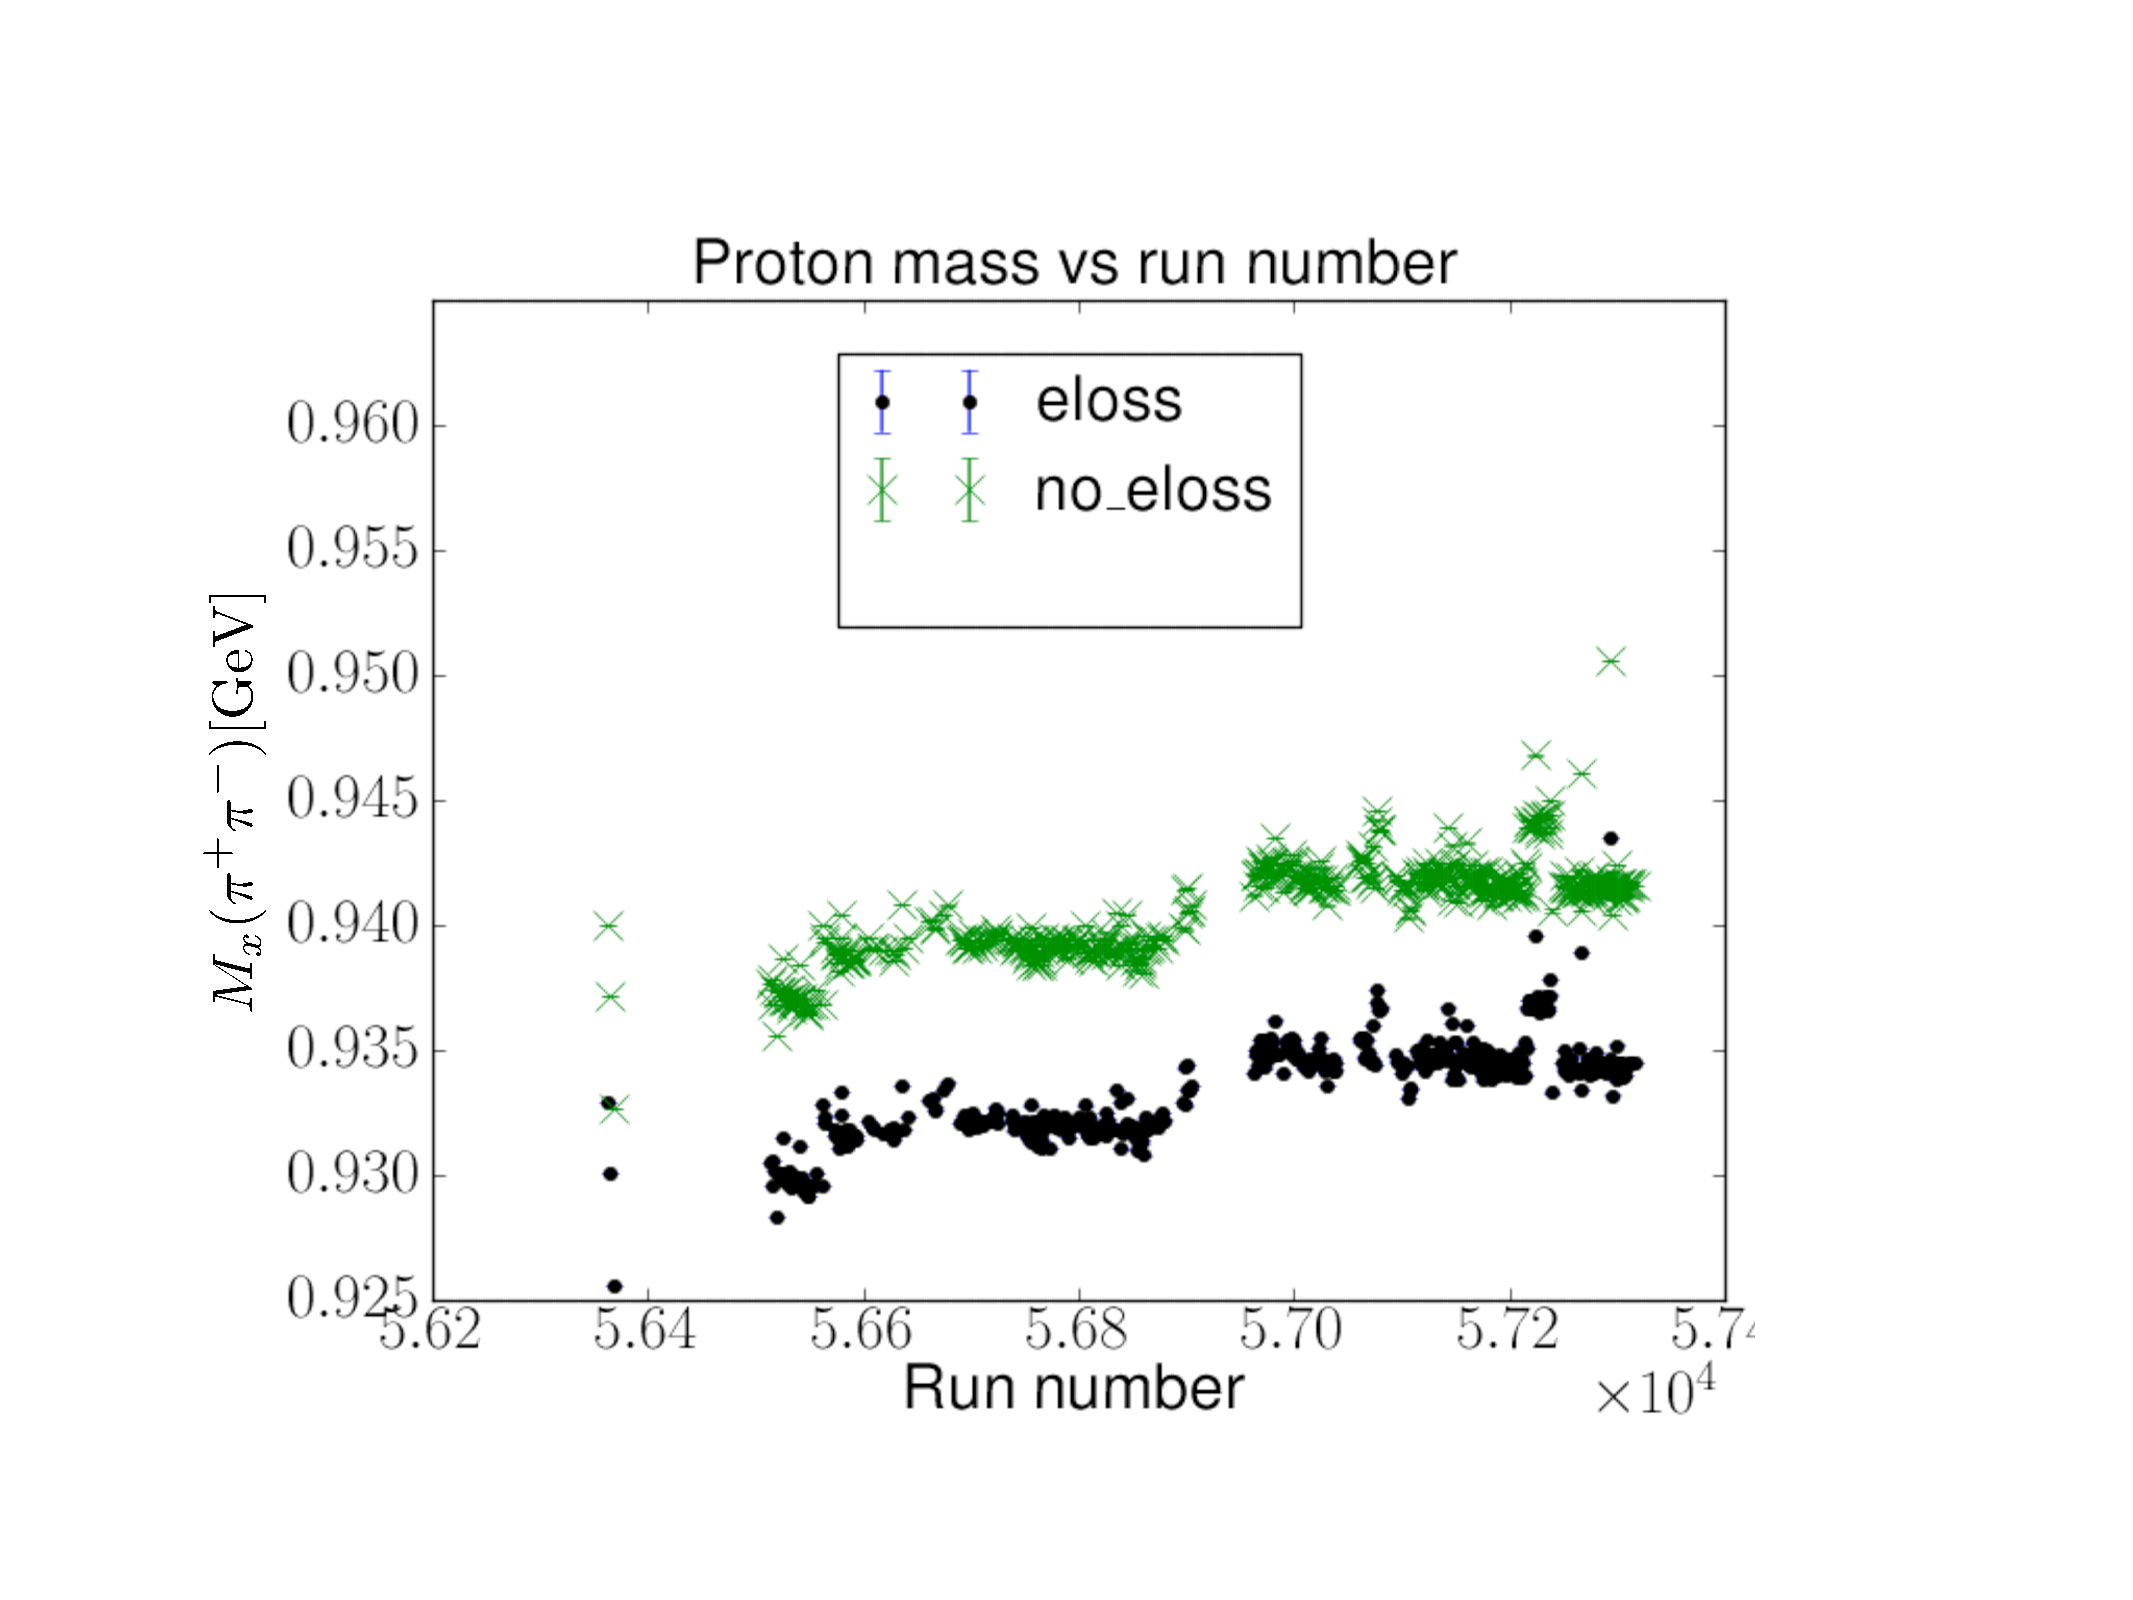
\includegraphics[width=\figwidth,height=0.75\hfigheight]{\figures/analysis/beam_correction/P_mass_issue.pdf}
\caption[Plot of \g12 run number vs. undetected proton mass with and without the ``energy-loss'' applied]{\label{fig:beamcor.p_mass}Plot of \g12 run number vs. undetected proton mass with and without the ``energy-loss'' applied. }
\end{center}\end{figure}

\begin{figure}[h!]\begin{center}
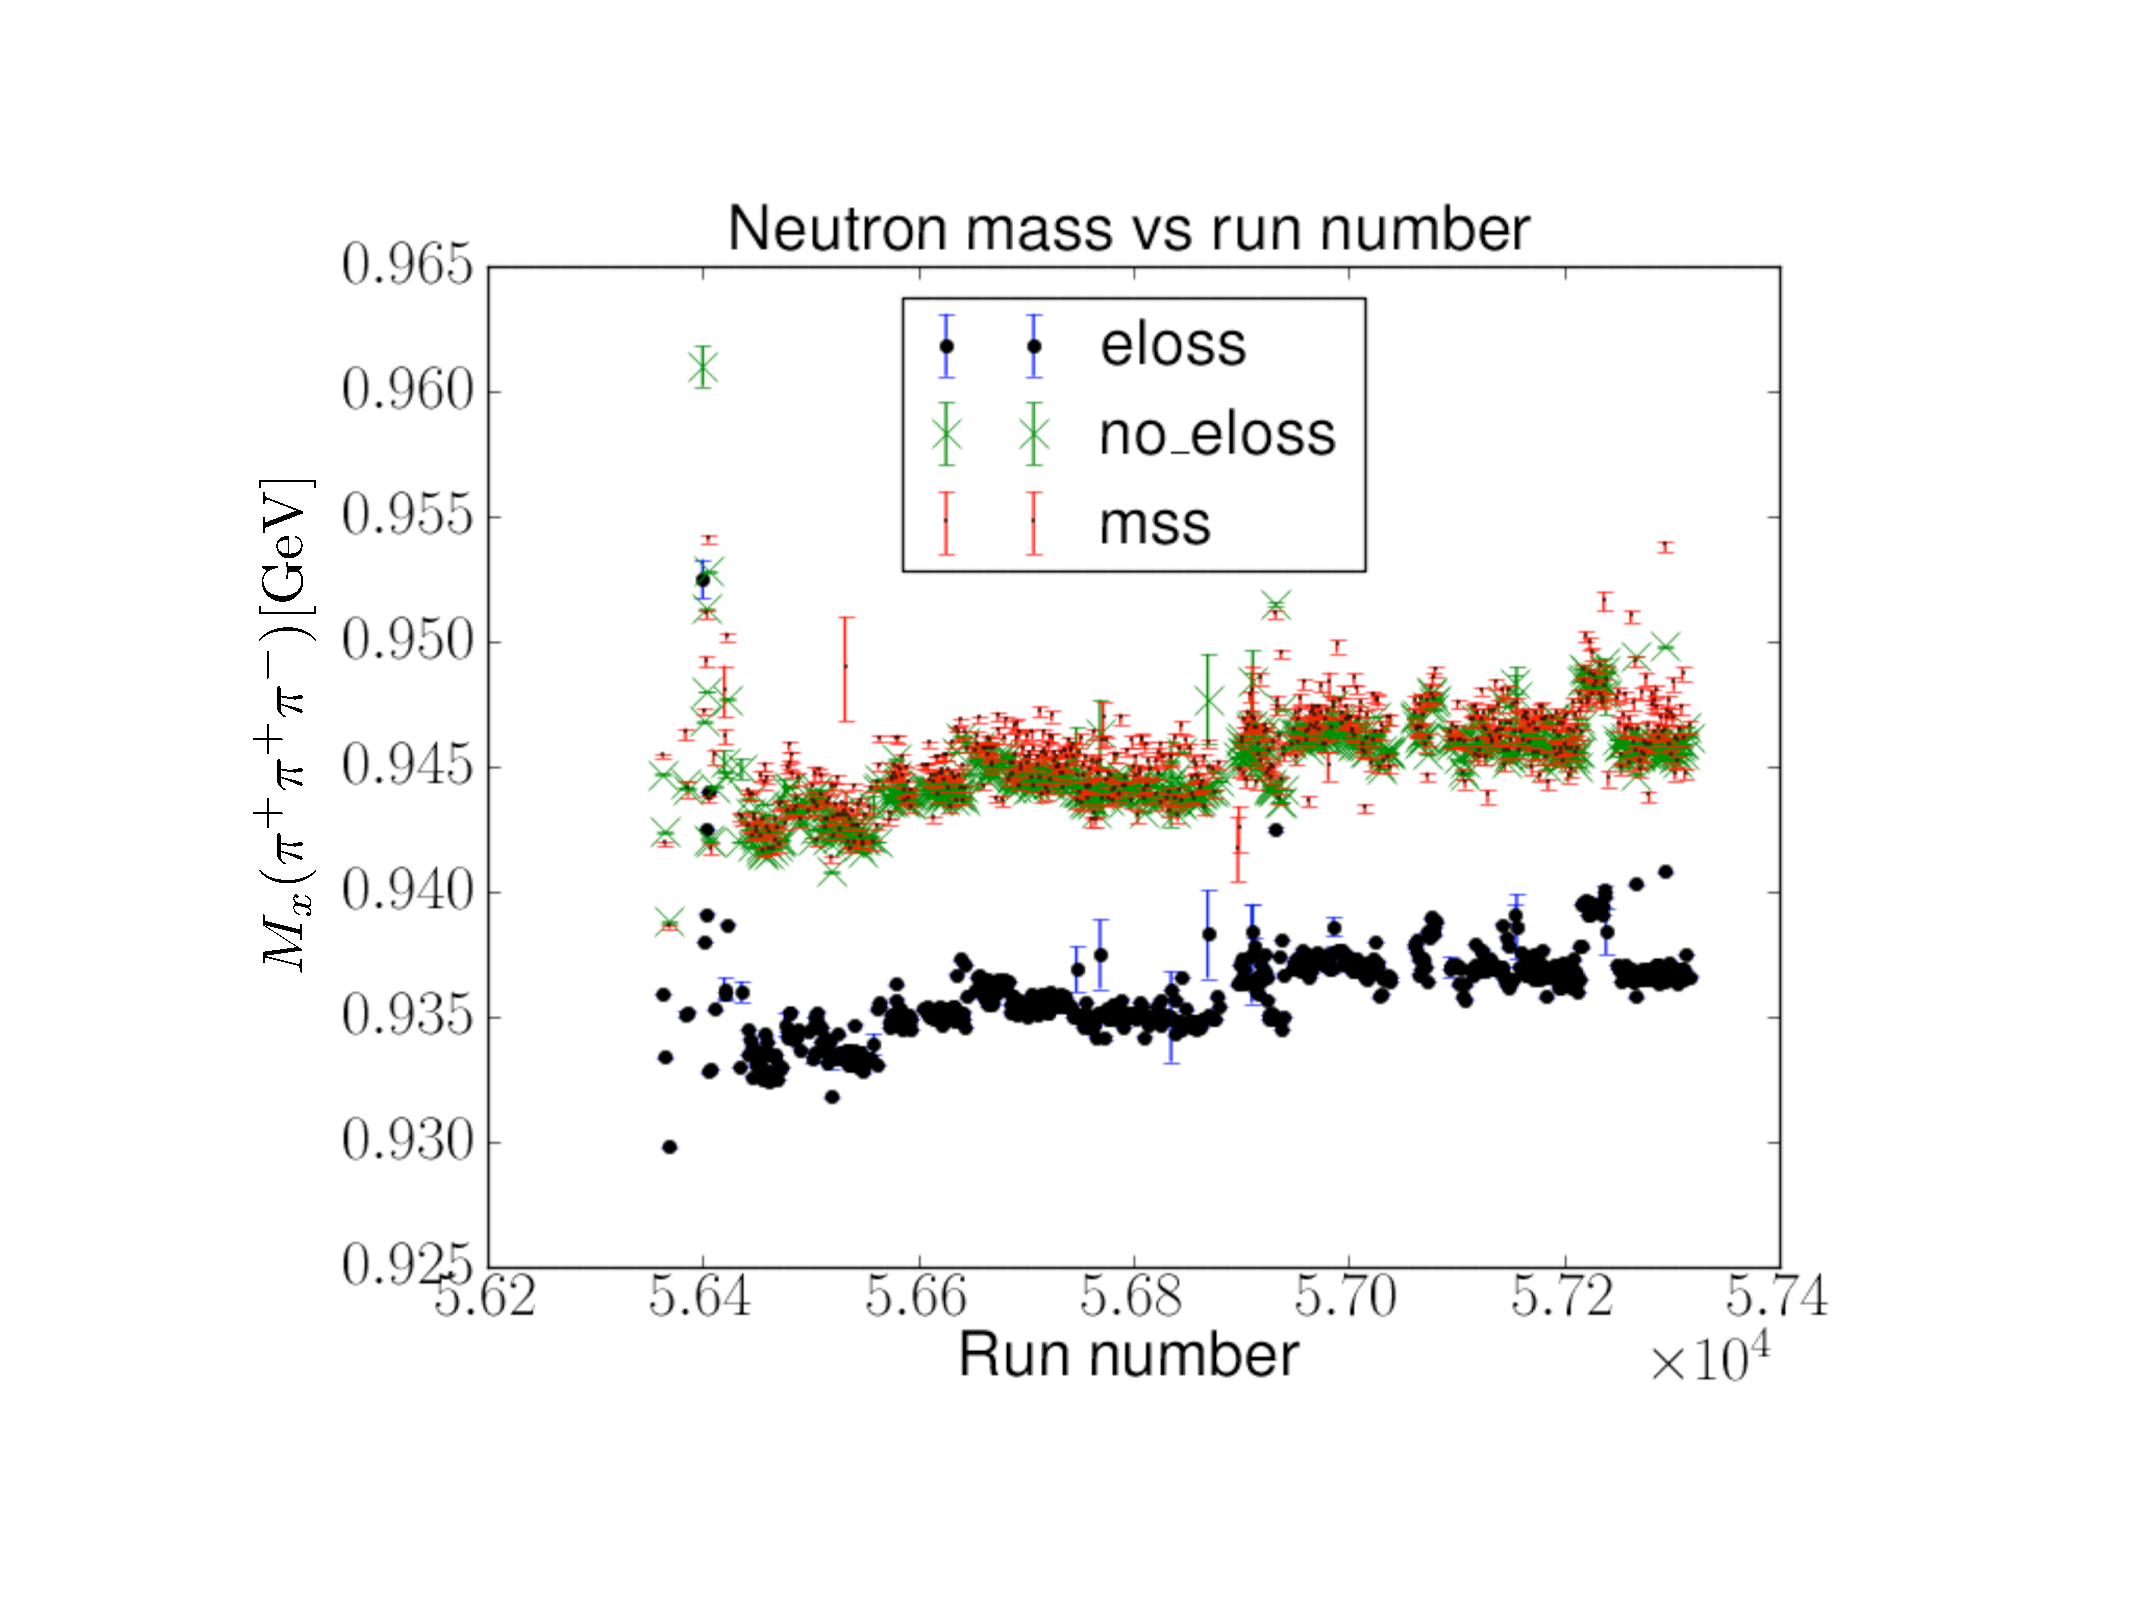
\includegraphics[width=\figwidth,height=0.75\hfigheight]{\figures/analysis/beam_correction/N_mass_issue.pdf}
\caption[Plot of \g12 run number vs. undetected neutron mass with and without the ``energy-loss'' applied]{\label{fig:beamcor.n_mass}Plot of \g12 run number vs. undetected neutron mass with and without the ``energy-loss'' applied. The red data points labeled ``mss" are data taken directly from tape. Image Source:~\cite{bookwalter}}
  \end{center}\end{figure}
  
  \begin{figure}[h!]\begin{center}
  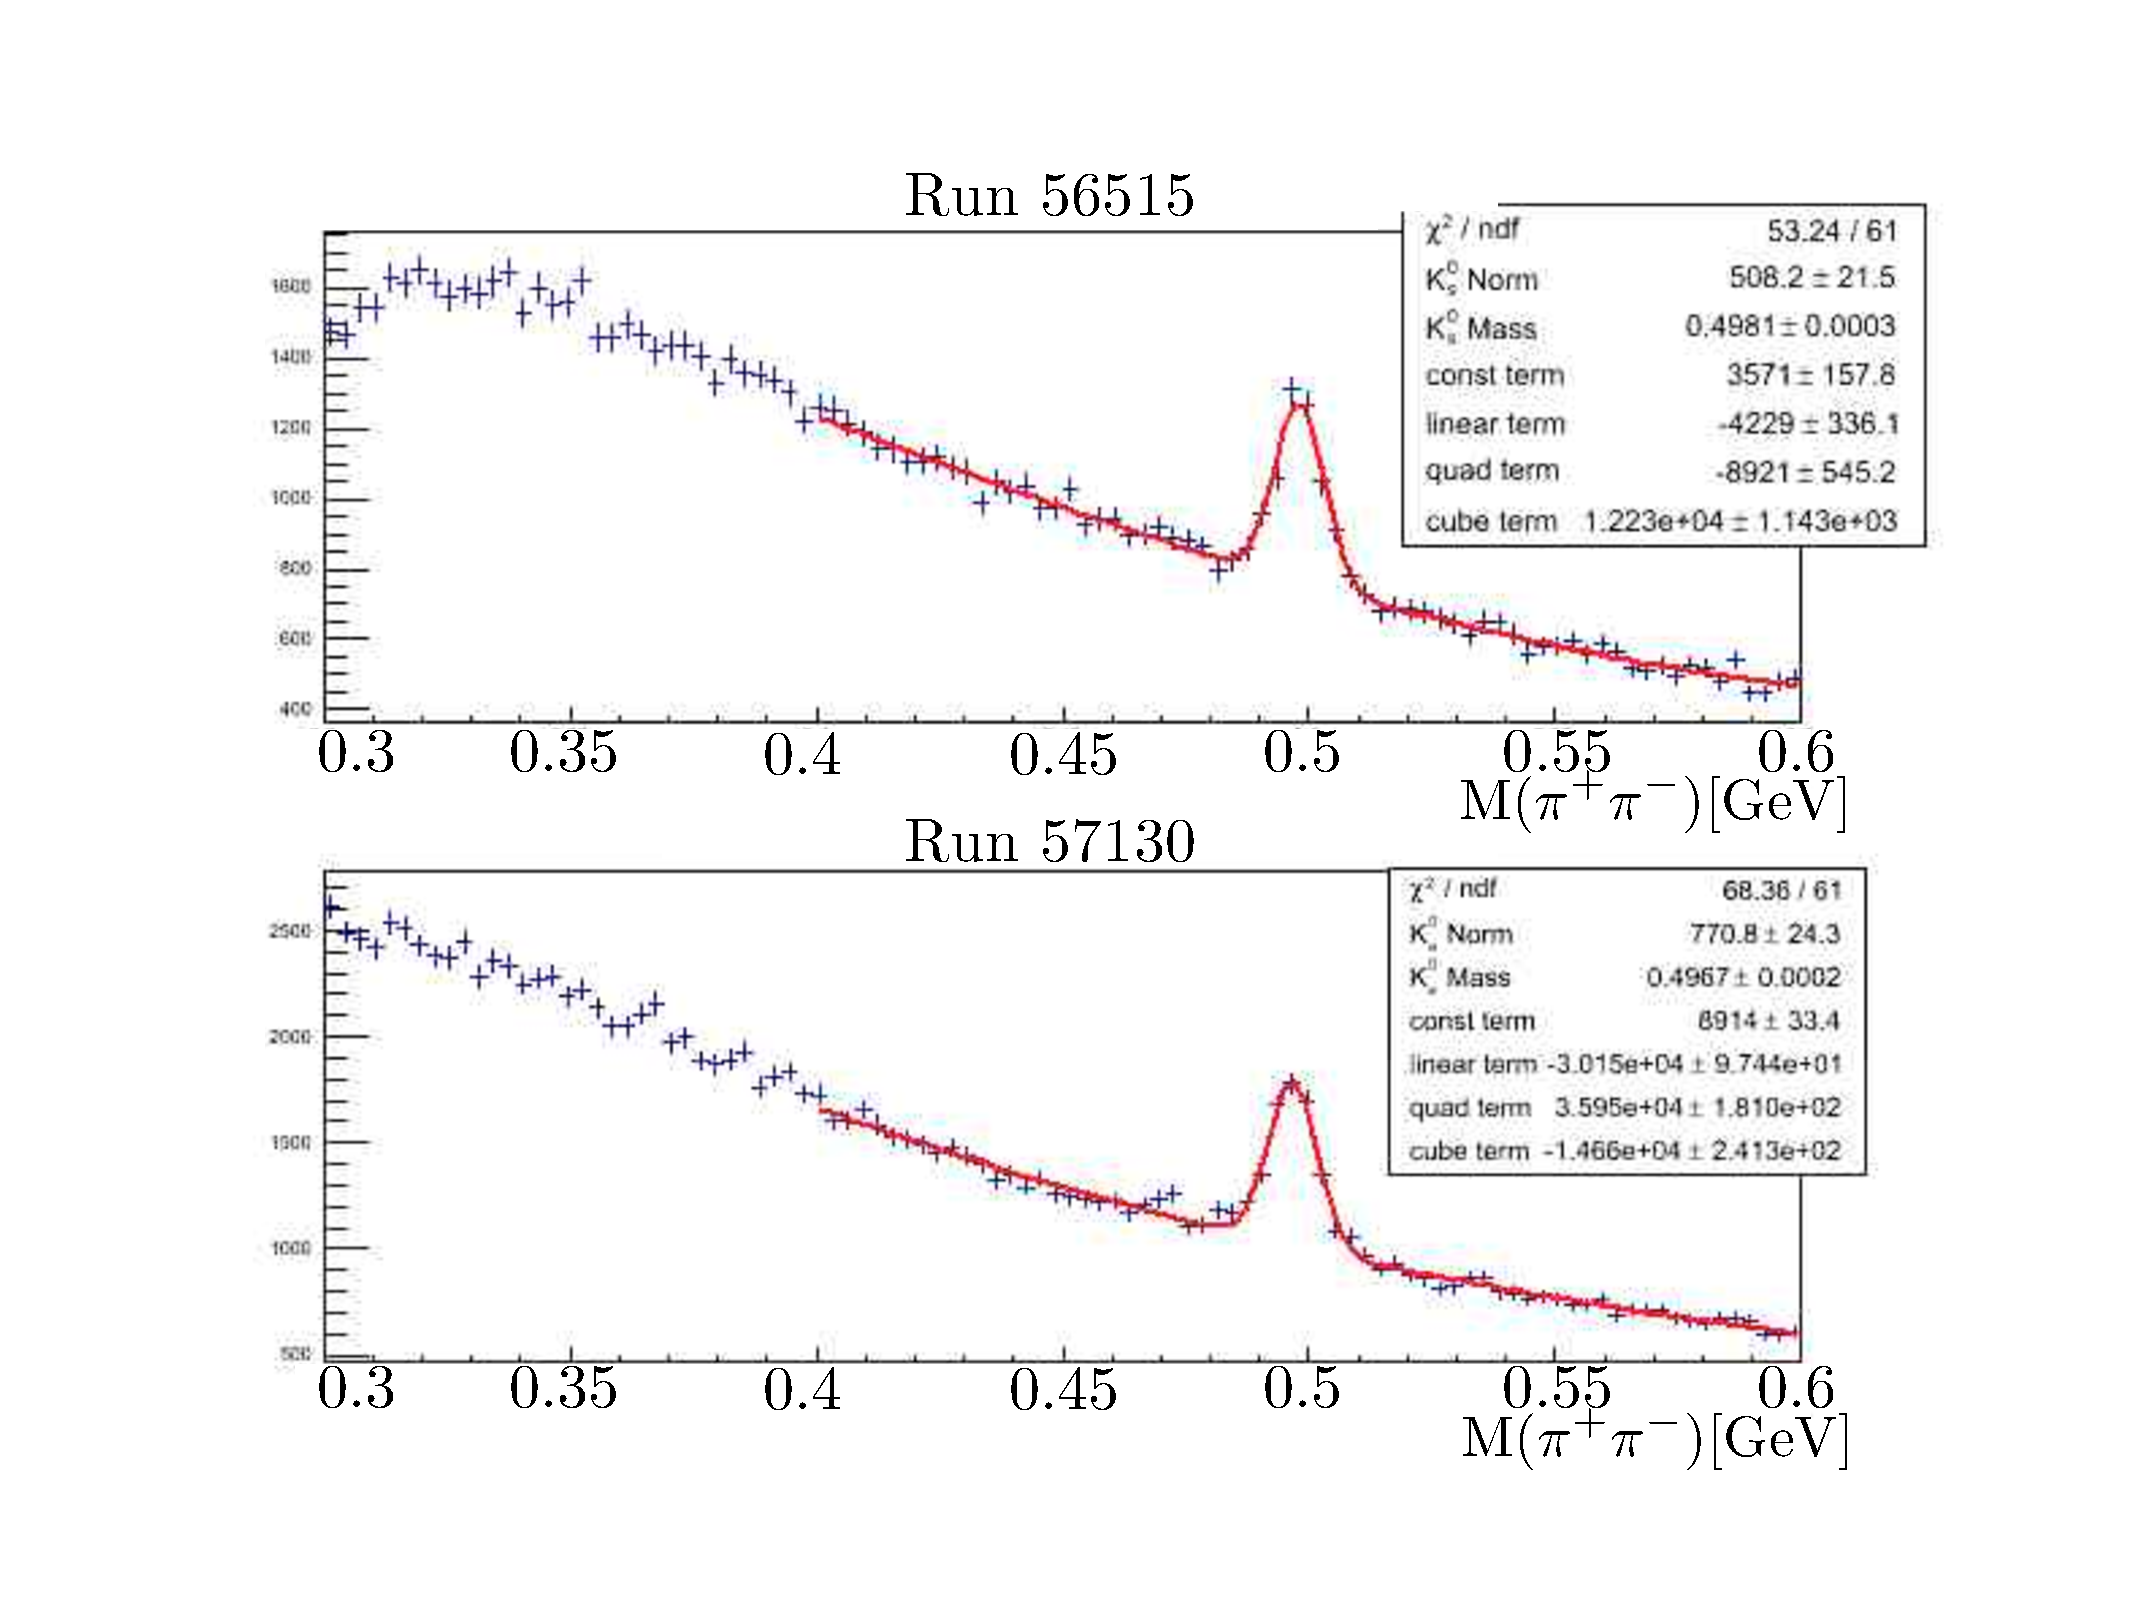
\includegraphics[width=\figwidth,height=0.7\hfigheight]{\figures/analysis/beam_correction/Kaon_mass.pdf}
  \caption[Plot of $\pi^+ \pi^-$ mass for runs 56515 and 57130]{\label{fig:beamcor.k_mass}Plot of $\pi^+ \pi^-$ mass for runs 56515 and 57130. $m_{K_0}$ = 0.4976 GeV/c$^2$.}
  \end{center}\end{figure}
  % % %
  \FloatBarrier
  Several tagger quantities were analyzed. The tagger magnet current was apparently constant (see Fig.~\ref{fig:tag.magnet.epics}) but had been turned off around run=56920 (May 12, 2008). When the tagger magnet was turned on, the current was set to its previous setting. The tagger magnet current was recorded by the accelerator group shown in Fig.~\ref{fig:tag.magnet.arne}, it was also stable throughout the running of \g12. The beam current was also stable (see Fig.~\ref{fig:beamcurrents})
  
  %Now that it is known that the photon beam energy is the cause of the issue, it must be known the cause of the photon beam error. Several quantities that the tagger subsystem are subjected to were analyzed, first being the tagger magnet current which, according to the \abbr{EPICS} Fig~\ref{fig:tag.magnet.epics}, remain constant
  %but showed that around run = 56920 (May 12, 2008) the tagger magnet was shut-off. The tagger magnet shut-off was done because work had to be done in the hall, however after the tagger magnet was turned on, the current was set to its previous setting. A further investigation into the tagger magnet was performed by private communication with the accelerator group chief Arne Freyberger, Fig~\ref{fig:tag.magnet.arne} shows the data the accelerator group had for the tagger magnet which confirms that the tagger magnet current was stable throughout the running of \g12. The next beam quantity analyzed was the beam current delivered by \abbr{CEBAF}, again through private communication with the accelerator group chief Arne Freyberger it is shown in Fig.~\ref{fig:beamcurrents} that the electron beam current remained constant throughout the \g12 experiment.
  
  \begin{figure}[h!]\begin{center}
  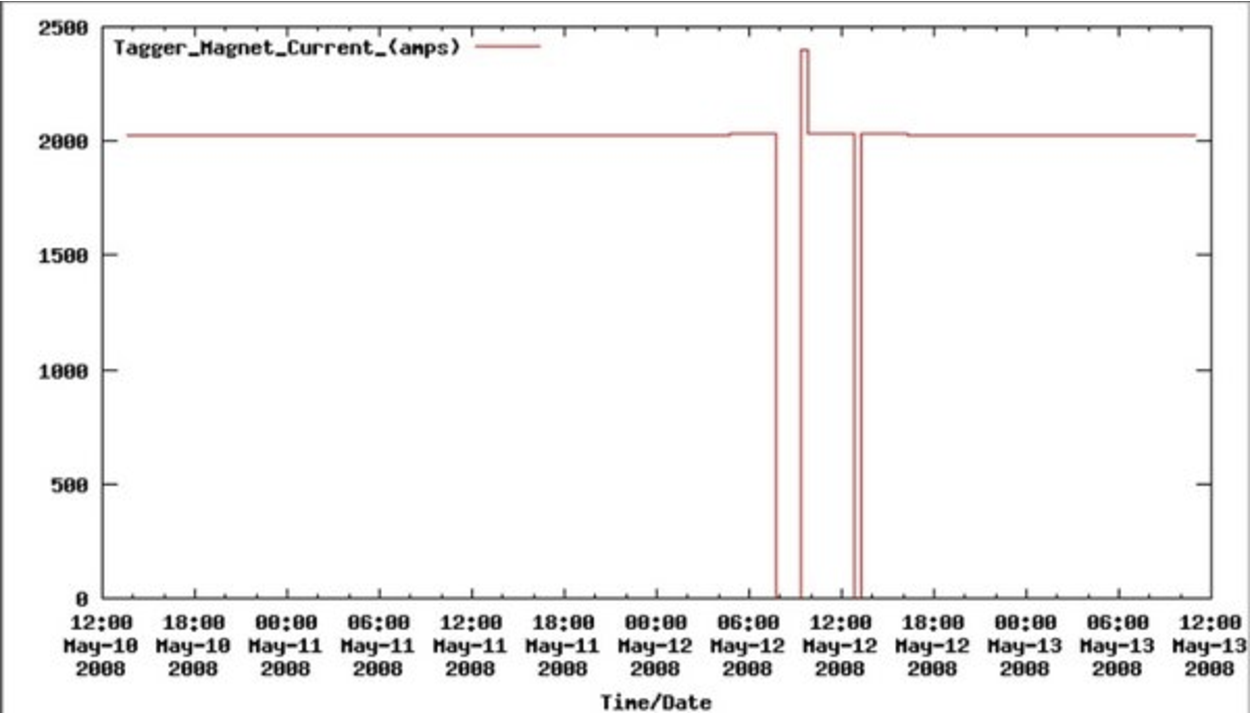
\includegraphics[width=\figwidth,height=0.7\hfigheight]{\figures/analysis/beam_correction/600px-Hystersis_smokingGun.pdf}
  \caption[Tagger magnet current according to \abbr{EPICS}]{\label{fig:tag.magnet.epics}Tagger magnet current according to \abbr{EPICS}}
  \end{center}\end{figure}
  
  \begin{figure}[h!]\begin{center}
  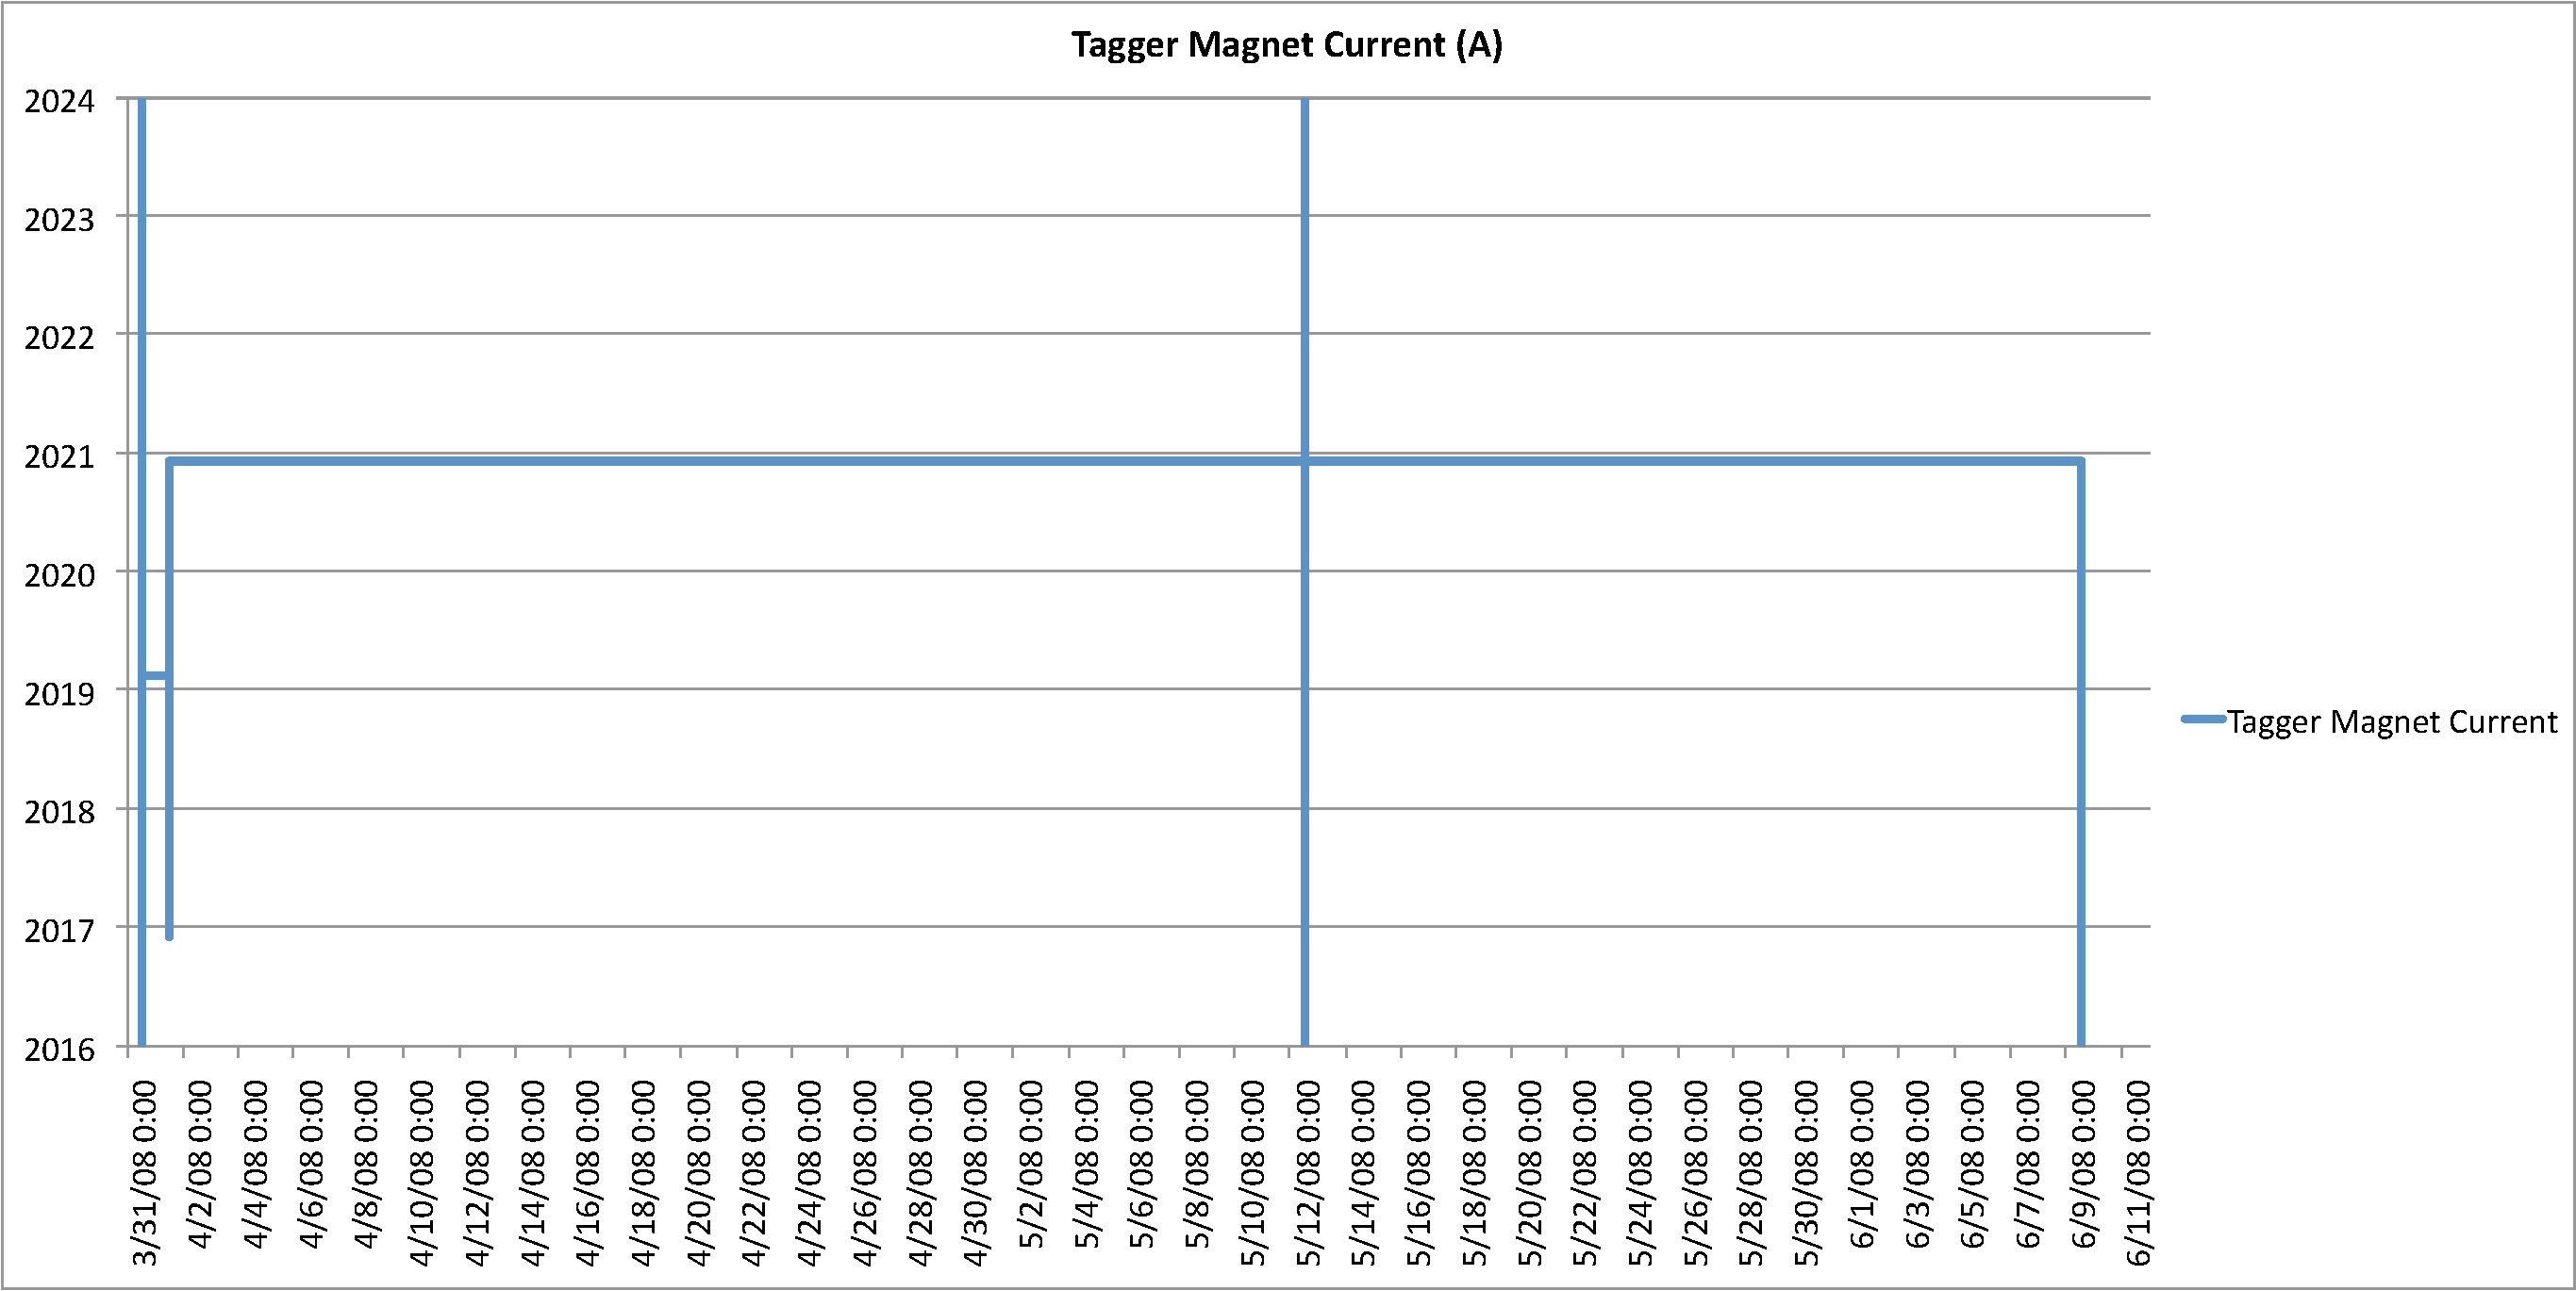
\includegraphics[width=\figwidth,height=0.7\hfigheight]{\figures/analysis/beam_correction/tagger_current_arne.pdf}
  \caption[Tagger magnet current according to accelerator group via \abbr{EPICS}]{\label{fig:tag.magnet.arne} Tagger magnet current according to accelerator group via \abbr{EPICS}}
  \end{center}\end{figure}
  
  \begin{figure}[h!]\begin{center}
  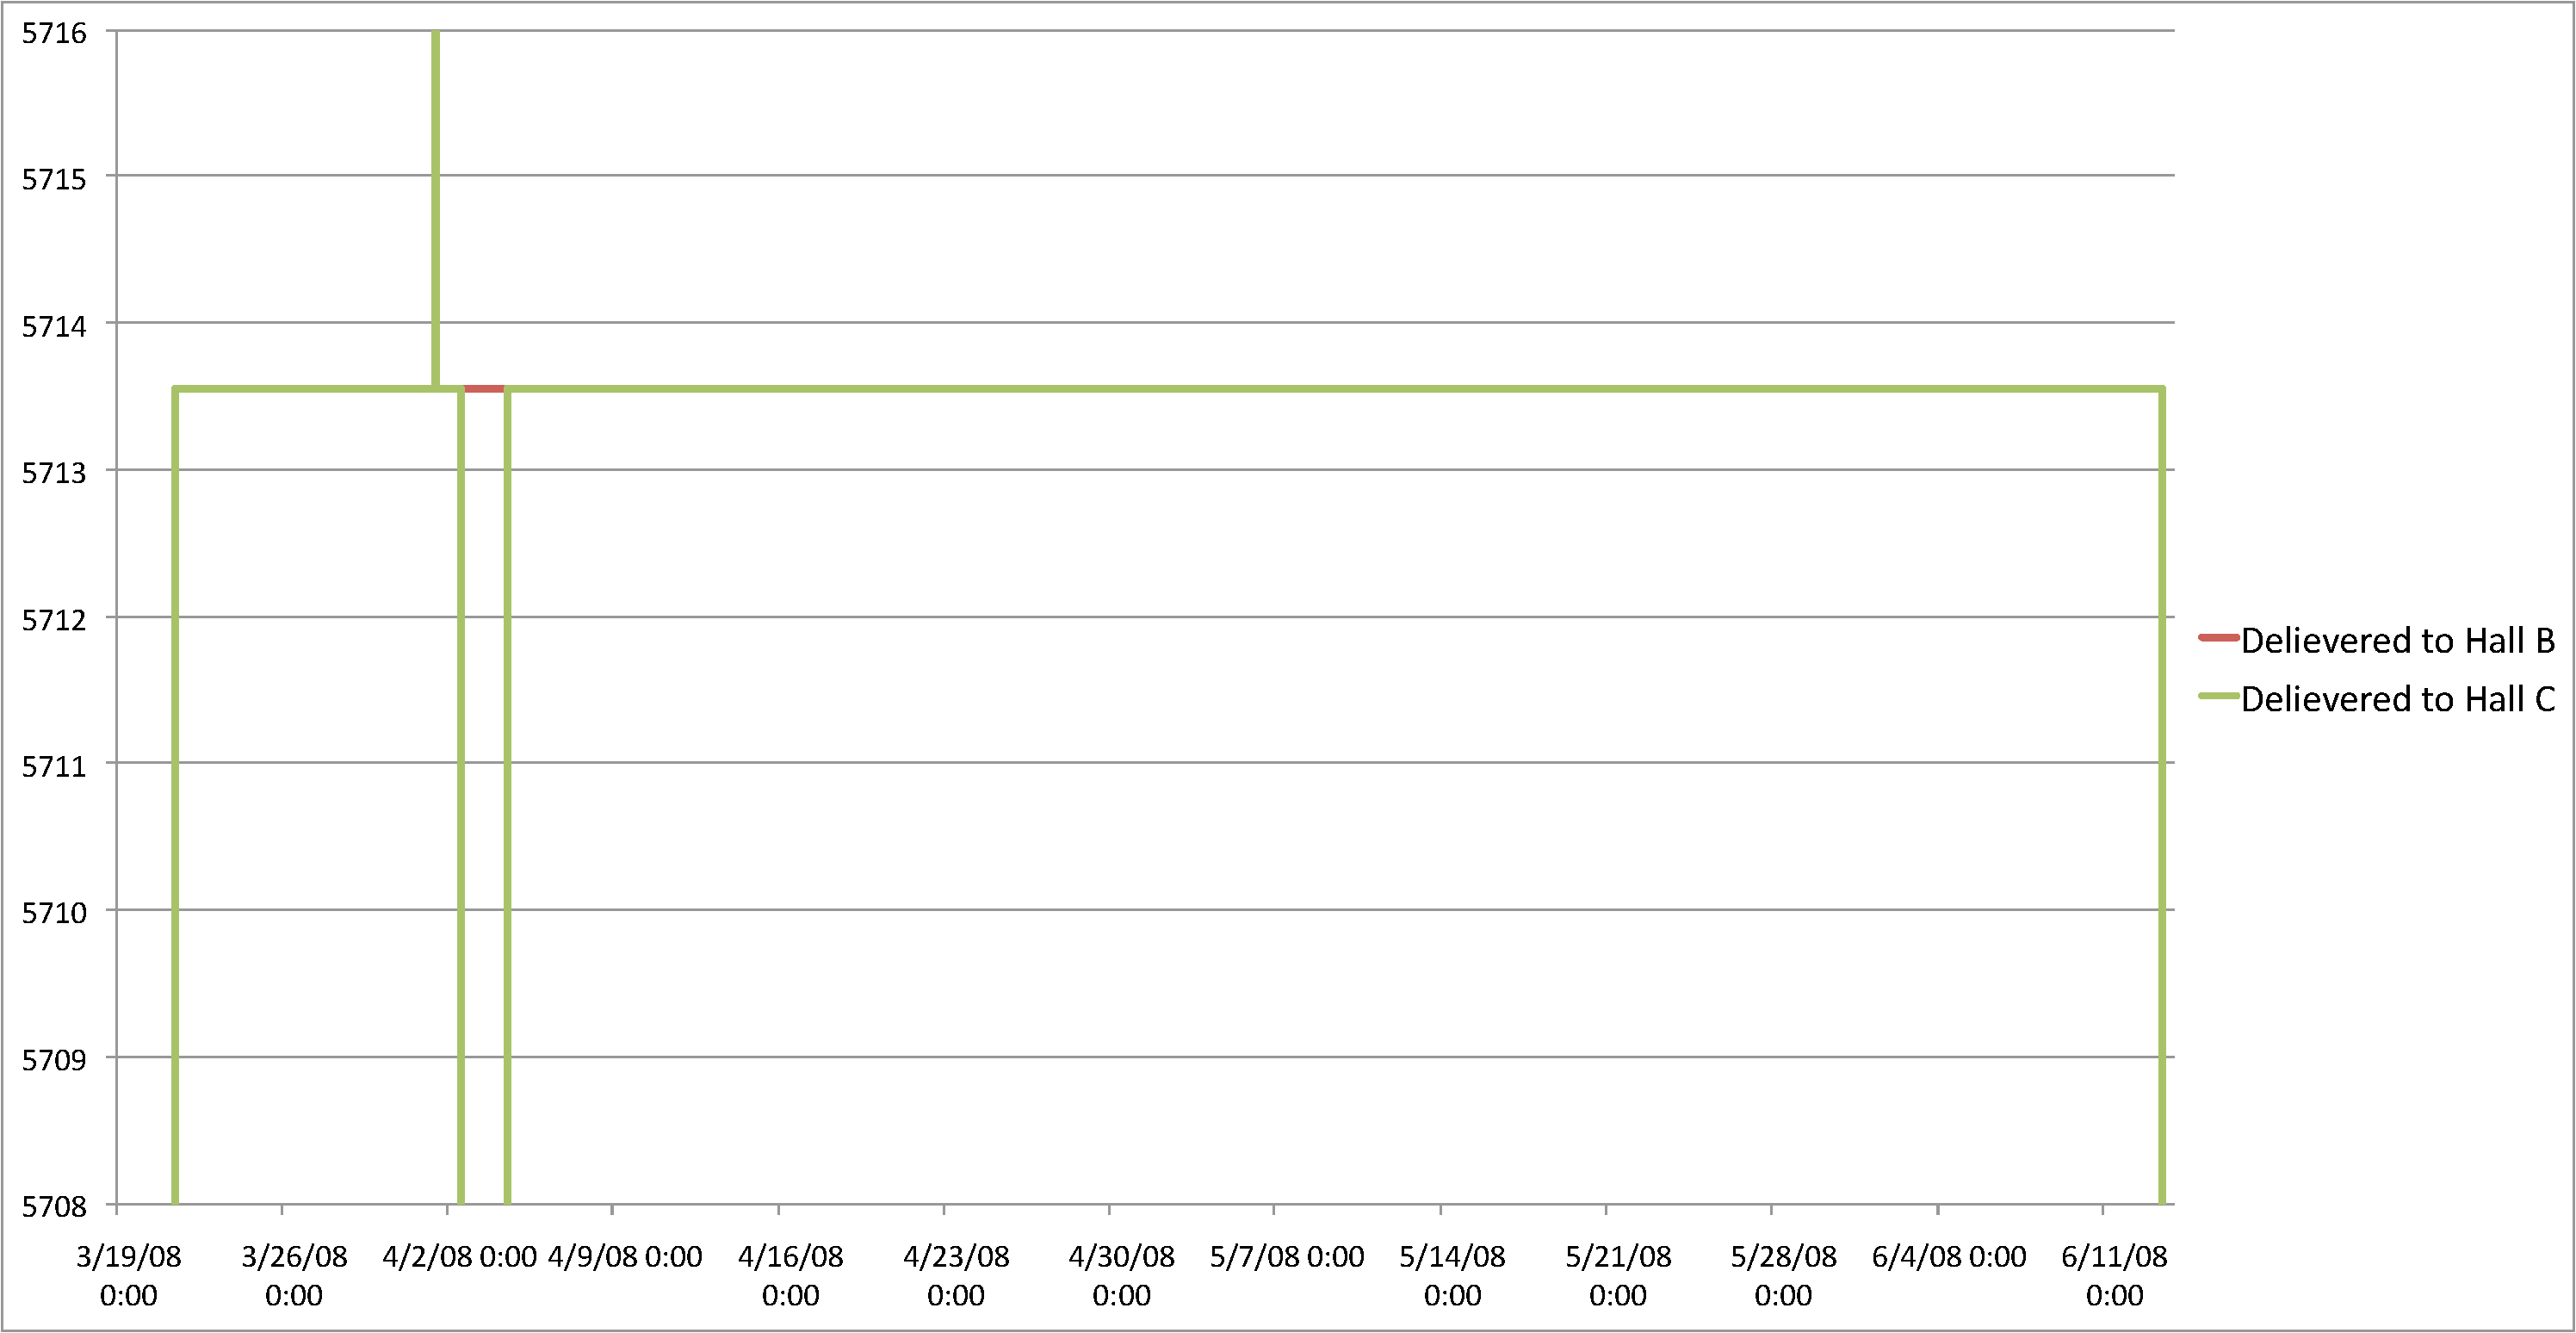
\includegraphics[width=\figwidth,height=0.7\hfigheight]{\figures/analysis/beam_correction/beam_currentsII.pdf}
  \caption[Electron beam current delivered to hall \desg{B}(red) and hall \desg{C} (green) according to the accelerator group during \g12]{\label{fig:beamcurrents}Electron beam current delivered to hall \desg{B}(red) and hall \desg{C} (green) according to the accelerator group during \g12. The green line overlays the red line except during the time around April, 03, 2008.}
  \end{center}\end{figure}
  
  The next quantity investigated was the positioning of the beam spot on the tagger dump. This quantity was used in place of the tagger magnetic field strength because hall \desg{B} does not measure the tagger magnetic field strength. However since the radius of curvature of a charged particle is inversely proportional to the magnetic field this quantity is suitable.
  \begin{equation}\label{eq:motioninmagII}
  p = qrB \ (\mathrm{if}\ \vec{p} \perp \vec{B} )
  \end{equation}
  The y-position of the tagger beam spot on the dump jumps on or about May 12, 2008 (see Fig.~\ref{fig:tagdump}). The change in y-position can only be due to the magnetic field changing. The phenomena in magnetism that allows for a steady current but a change in magnetic field is known as hysteresis (see Fig.~\ref{fig:hyst}).
    \begin{figure}[h!]\begin{center}
  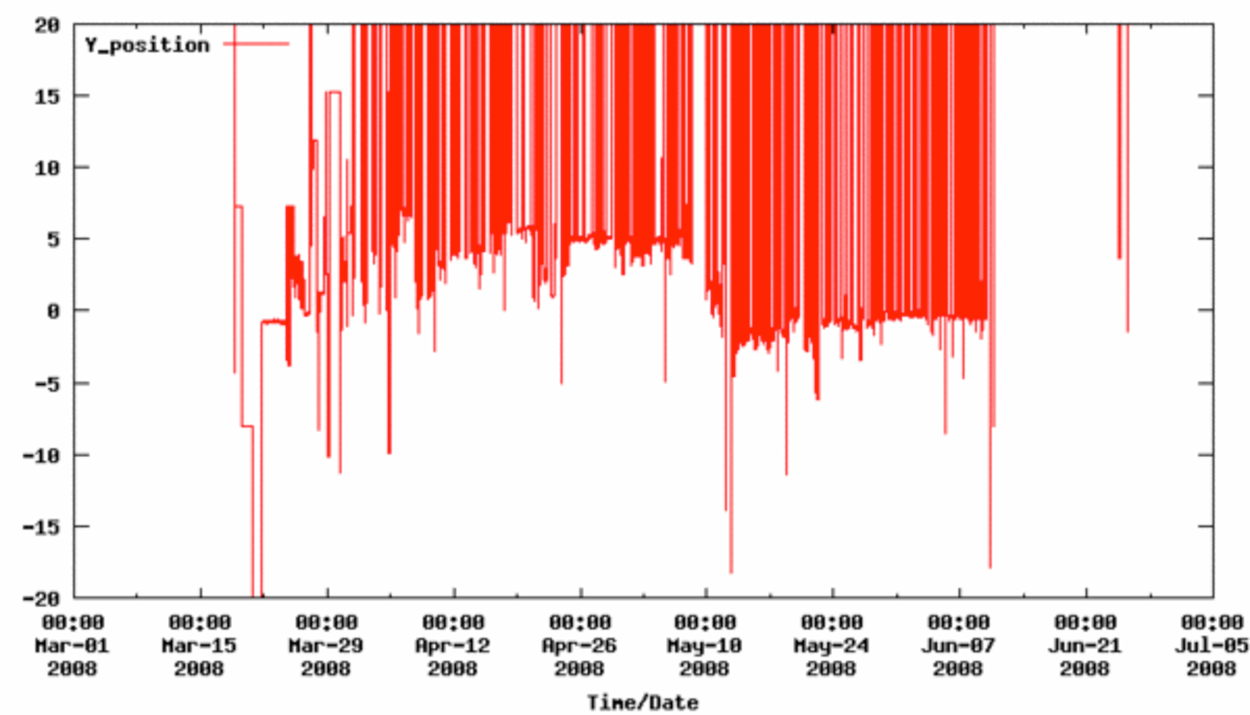
\includegraphics[width=\figwidth,height=0.7\hfigheight]{\figures/analysis/beam_correction/600px-Tagger-dump-y.pdf}
  \caption[Tagger dump beam spot y-position according to \abbr{EPICS}]{\label{fig:tagdump}Tagger dump beam spot y-position according to \abbr{EPICS}}
  \end{center}\end{figure}
  
  \begin{figure}[h!]\begin{center}
  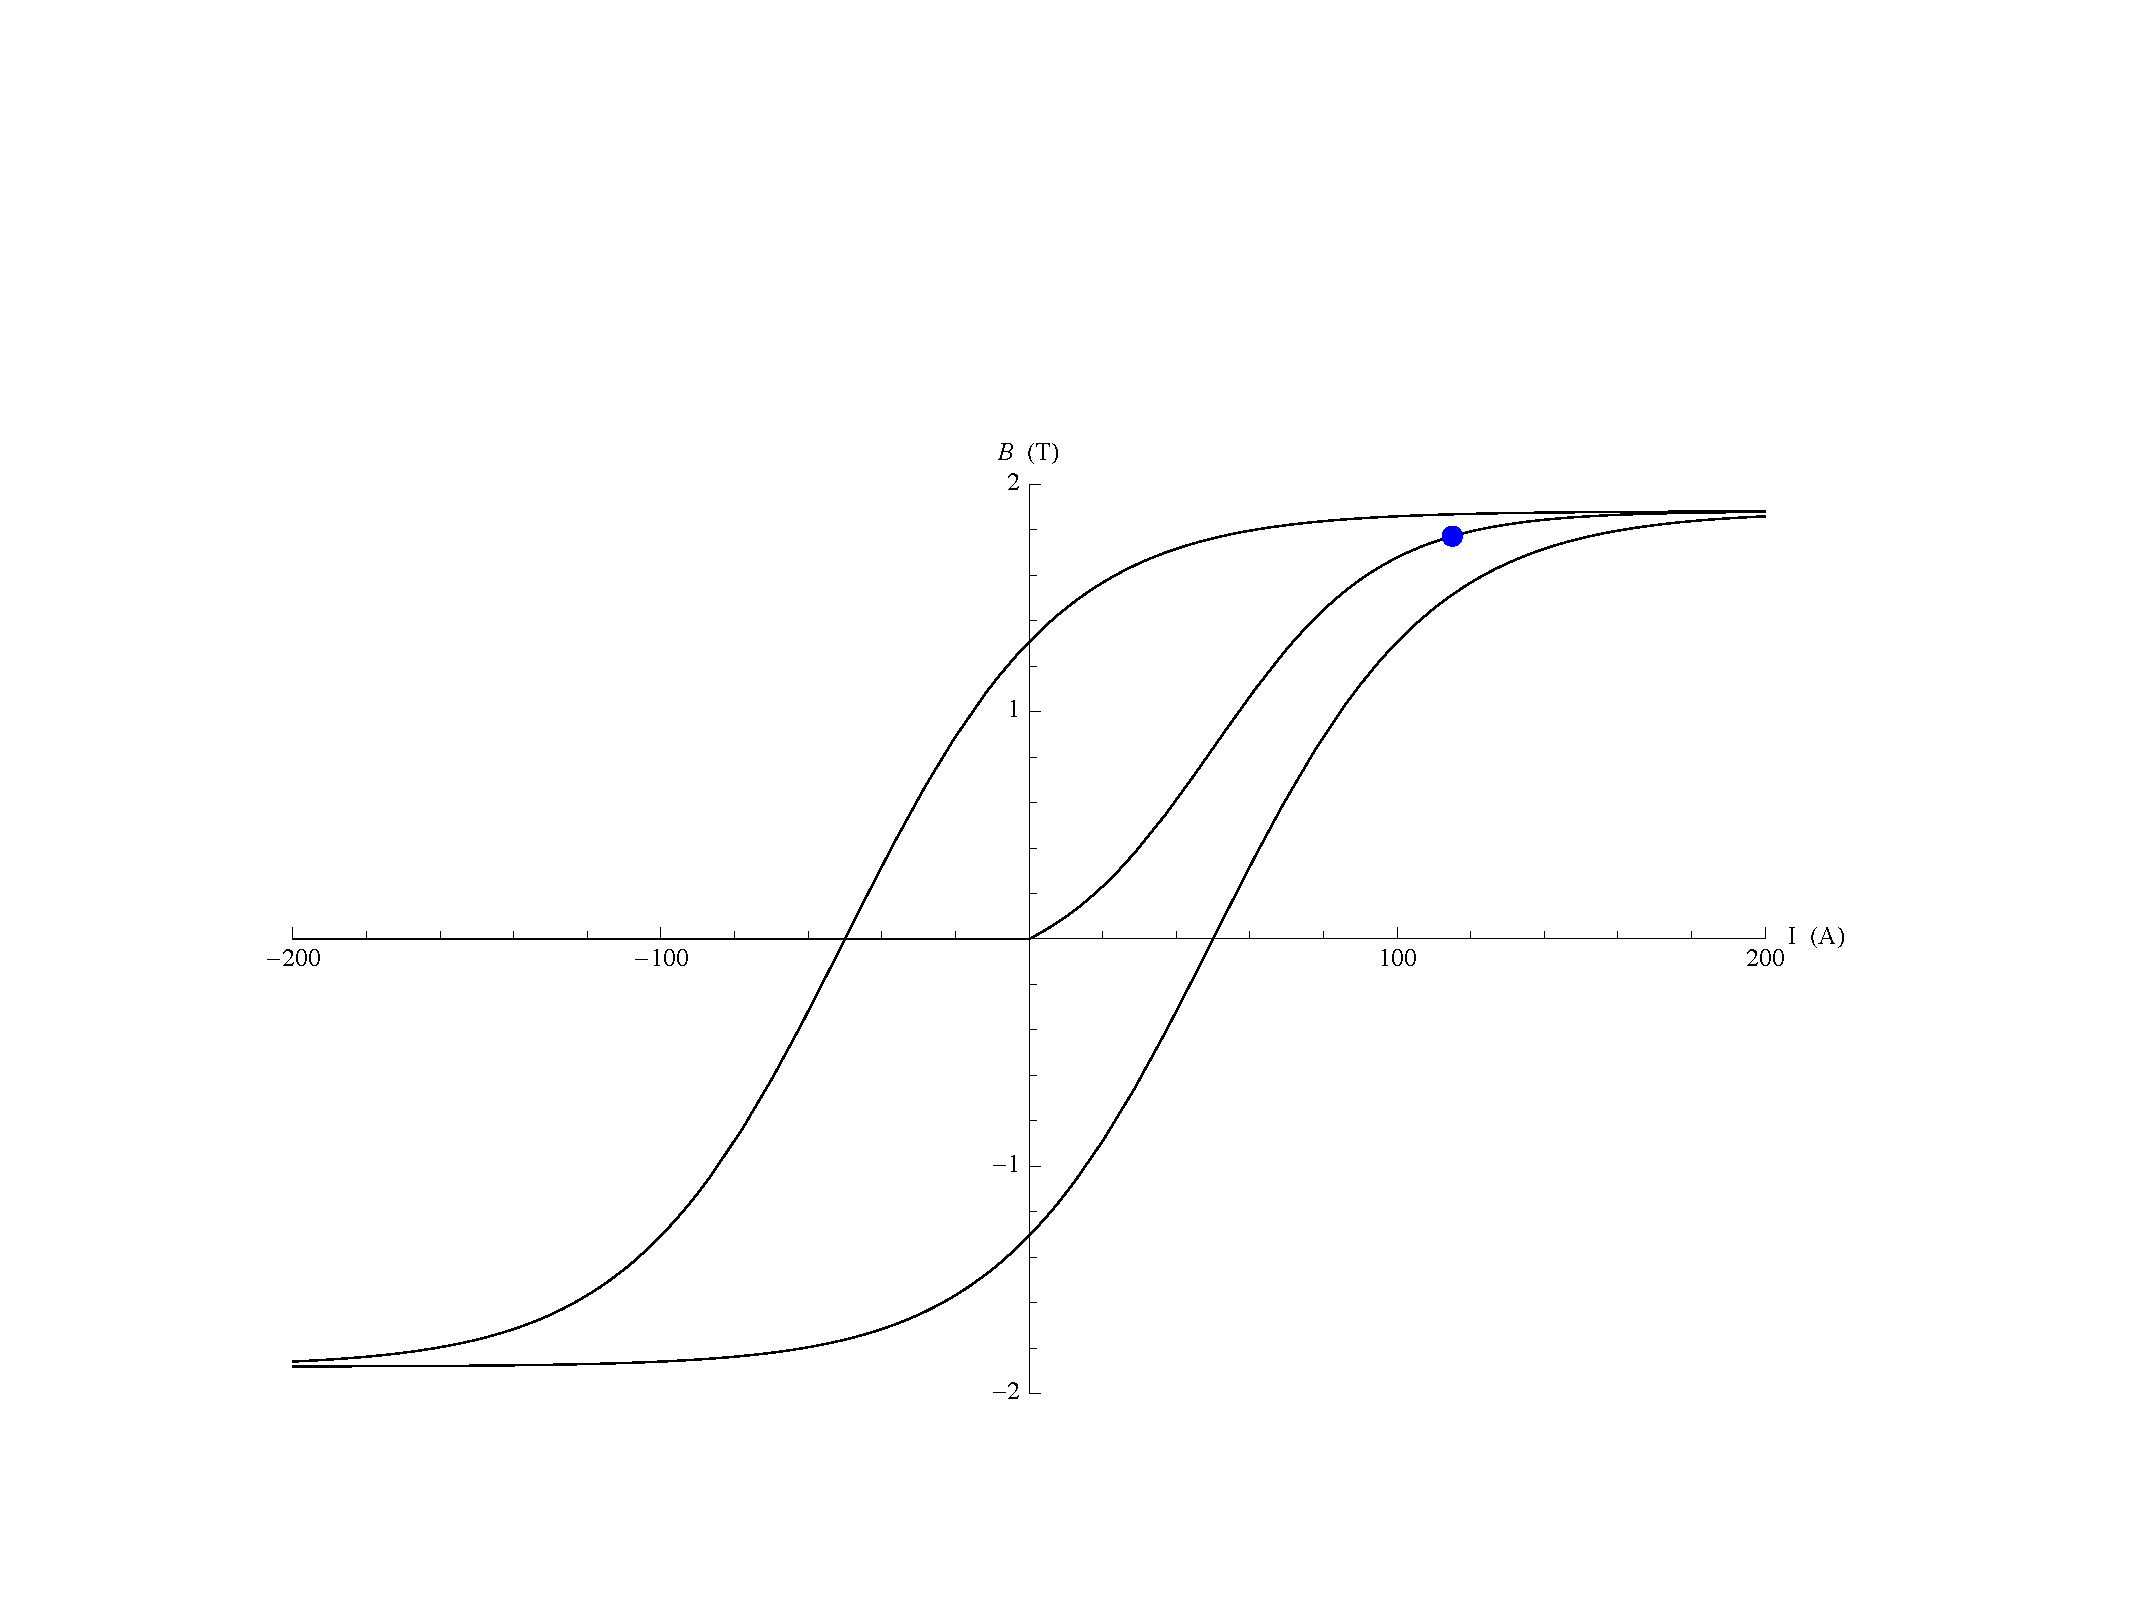
\includegraphics[width=\figwidth,height=0.7\hfigheight]{\figures/analysis/beam_correction/hysteresis_keynote.pdf}
  \caption[Plot depicting magnetic field strength vs. magnet current showing the process of hysteresis]{\label{fig:hyst}Plot depicting magnetic field strength vs. magnet current showing the process of hysteresis. For a current of strength I, there could exist many magnetic fields of strength B.}
  \end{center}\end{figure}
  \FloatBarrier
  It appeared that the \g12 missing mass fluctuations are due to tagger magnet hysteresis and the effect it would be on the scattered electron nd hence the tagged photon. The tagged photon energies were corrected as follows;
  \begin{align}
  P_{\pi^+} + P_{\pi^-} = P_{\pi^+ \pi^-} \nonumber
  \end{align}
  where $P_{\pi^+}$, $P_{\pi^-}$ are the 4-momenta of the $\pi^+$, $\pi^-$ respectively and $P_{\pi^+ \pi^-}$ is the sum of $\pi^+$ and $\pi^-$ 4-momenta.
  Therefore;
  \begin{align}
  &(P_{\gamma} + P_{target} - (P_{\pi^+\pi^-}))^2 = m_p^2 \\
  & P_{\gamma}^2 + P_{target}^2 + P_{\pi^+\pi^-}^2 + 2P_{\gamma}P_{target} - 2P_{\gamma}P_{\pi^+\pi^-} - 2P_{target}P_{\pi^+\pi^-}= m_p^2
  \end{align}
  collecting terms of $P_{\gamma}$ to one side and using $P_{target}^2 = m_p^2 $ and $P_{\gamma}^2 = 0$
  \begin{align}\label{eq:hyst.eqI}
  P_{\pi^+\pi^-}^2 - 2P_{target}P_{\pi^+\pi^-}= 2P_{\gamma}(P_{\pi^+\pi^-} - P_{target})
  \end{align}
  From this using Eq.~\ref{eq:tagger.energy} in 4-vector notation
  \begin{align}\label{eq:tagger.energyII}
  P_{\gamma} = P_{E_0} - P_{e}\nonumber
  \end{align}
  where $P_{E_0}$ is the four vector of the incident electron and $P_{e}$ is the four vector of the scattered electron in the bremsstrahlung process that is measured by the tagger. Applying a scaler correction to $P_{e}$ as $xP_{e}$ and solving for $x$ for all known quantities, Eq.~\ref{eq:hyst.eqI} simplifies to;
  \begin{align}
  x= \frac{P_{E_0}(P_{target}-P_{\pi^+\pi^-}) + P_{\pi^+\pi^-}^2/2  - P_{target}P_{\pi^+\pi^-}}{(P_{E_0} - P_{\gamma})(P_{target} - P_{\pi^+\pi^-})}
  \end{align}
  To reduce statistical fluctuations $\frac{1}{10}$ of run 56515 was analyzed to obtain the correction factor $x$. The correction factor was fitted using a Gaussian to establish an accurate measurement of the peak, this is shown in Fig~\ref{fig:56515.cor}. After the correction factor was extracted for run 56515, it was applied to both the reactions listed in Eq.~\ref{eq:beam.cortopology} and Eq.~\ref{eq:beam.checktopology} by recalculating the photon beam energy as;
  \begin{align}
  E_e = E_{E_0} - E_{\gamma} \nonumber \\
  E_{\gamma}^{new} = E_{E_0} - xE_e \nonumber.
  \end{align}
  Figures~\ref{fig:proton.fix},~\ref{fig:neutron.fix} illustrate the missing masses after the tagger correction and show that the new calculated missing masses are less than 1~MeV from \abbr{PDG} values. Since both the missing proton mass and missing neutron mass were adjusted properly to the correct mass by using the same beam correction factor, it shows that the correction factor is independent of reaction and therefore can be applied to all \g12 analyses. The procedure to calculate $x$ was repeated for every run in \g12, Fig~\ref{fig:beamcor.run}, with $\frac{1}{10}$ of the data used. To validate the corrections of the entire \g12 data set, the missing neutron mass was recalculated for each run, shown in  Fig.~\ref{fig:neutron.fixall}, using several correction schemes, i.e. a scheme of just ``energy-loss'' corrections, a scheme of ``energy-loss'' and momentum corrections (JTG PCor), a scheme of ``energy-loss'', momentum corrections (JTG PCor) and beam corrections (MK BeamCor) and a scheme of ``energy-loss'' and beam corrections (MK BeamCor). It can be seen in Fig.~\ref{fig:neutron.fixall} that the only scheme that sufficed was the combination of ``energy-loss'' and beam corrections.
  
  
  \begin{figure}[h!]\begin{center}
  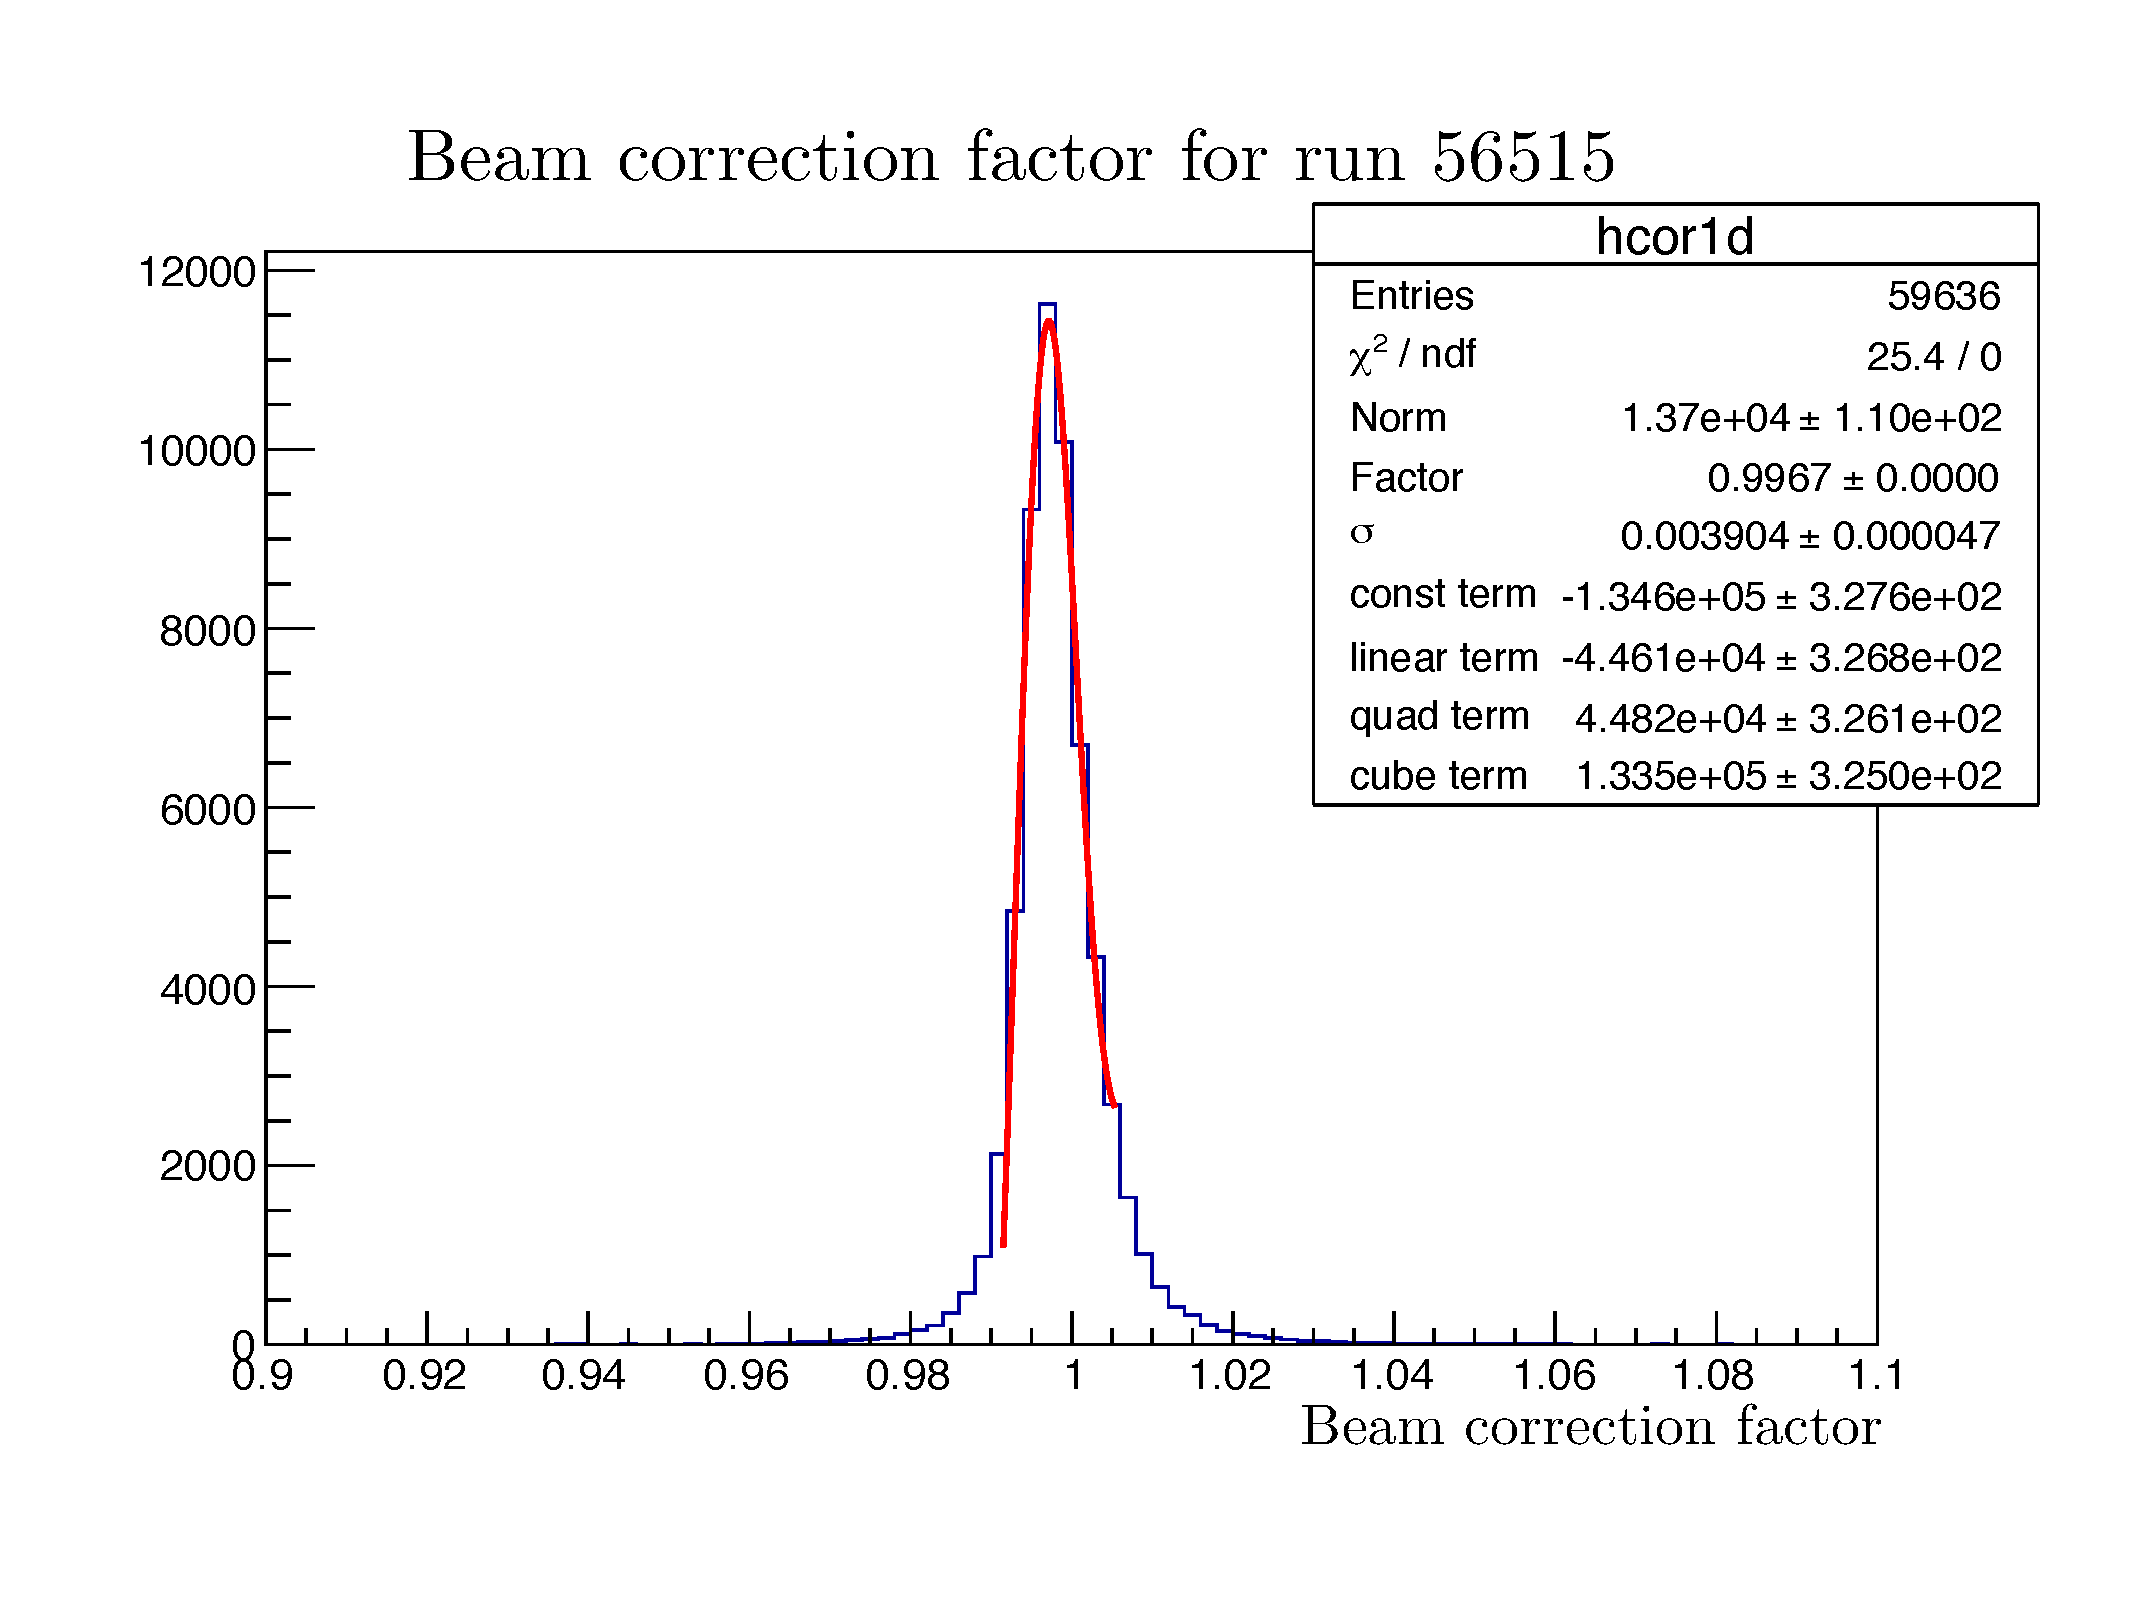
\includegraphics[width=\figwidth,height=0.7\hfigheight]{\figures/analysis/beam_correction/56515_cor.pdf}
  \caption[Beam correction factor for run 56515]{\label{fig:56515.cor} Beam correction factor for run 56515. The fit is a Gaussian function.}
    \end{center}\end{figure}
    
    \begin{figure}[h!]\begin{center}
    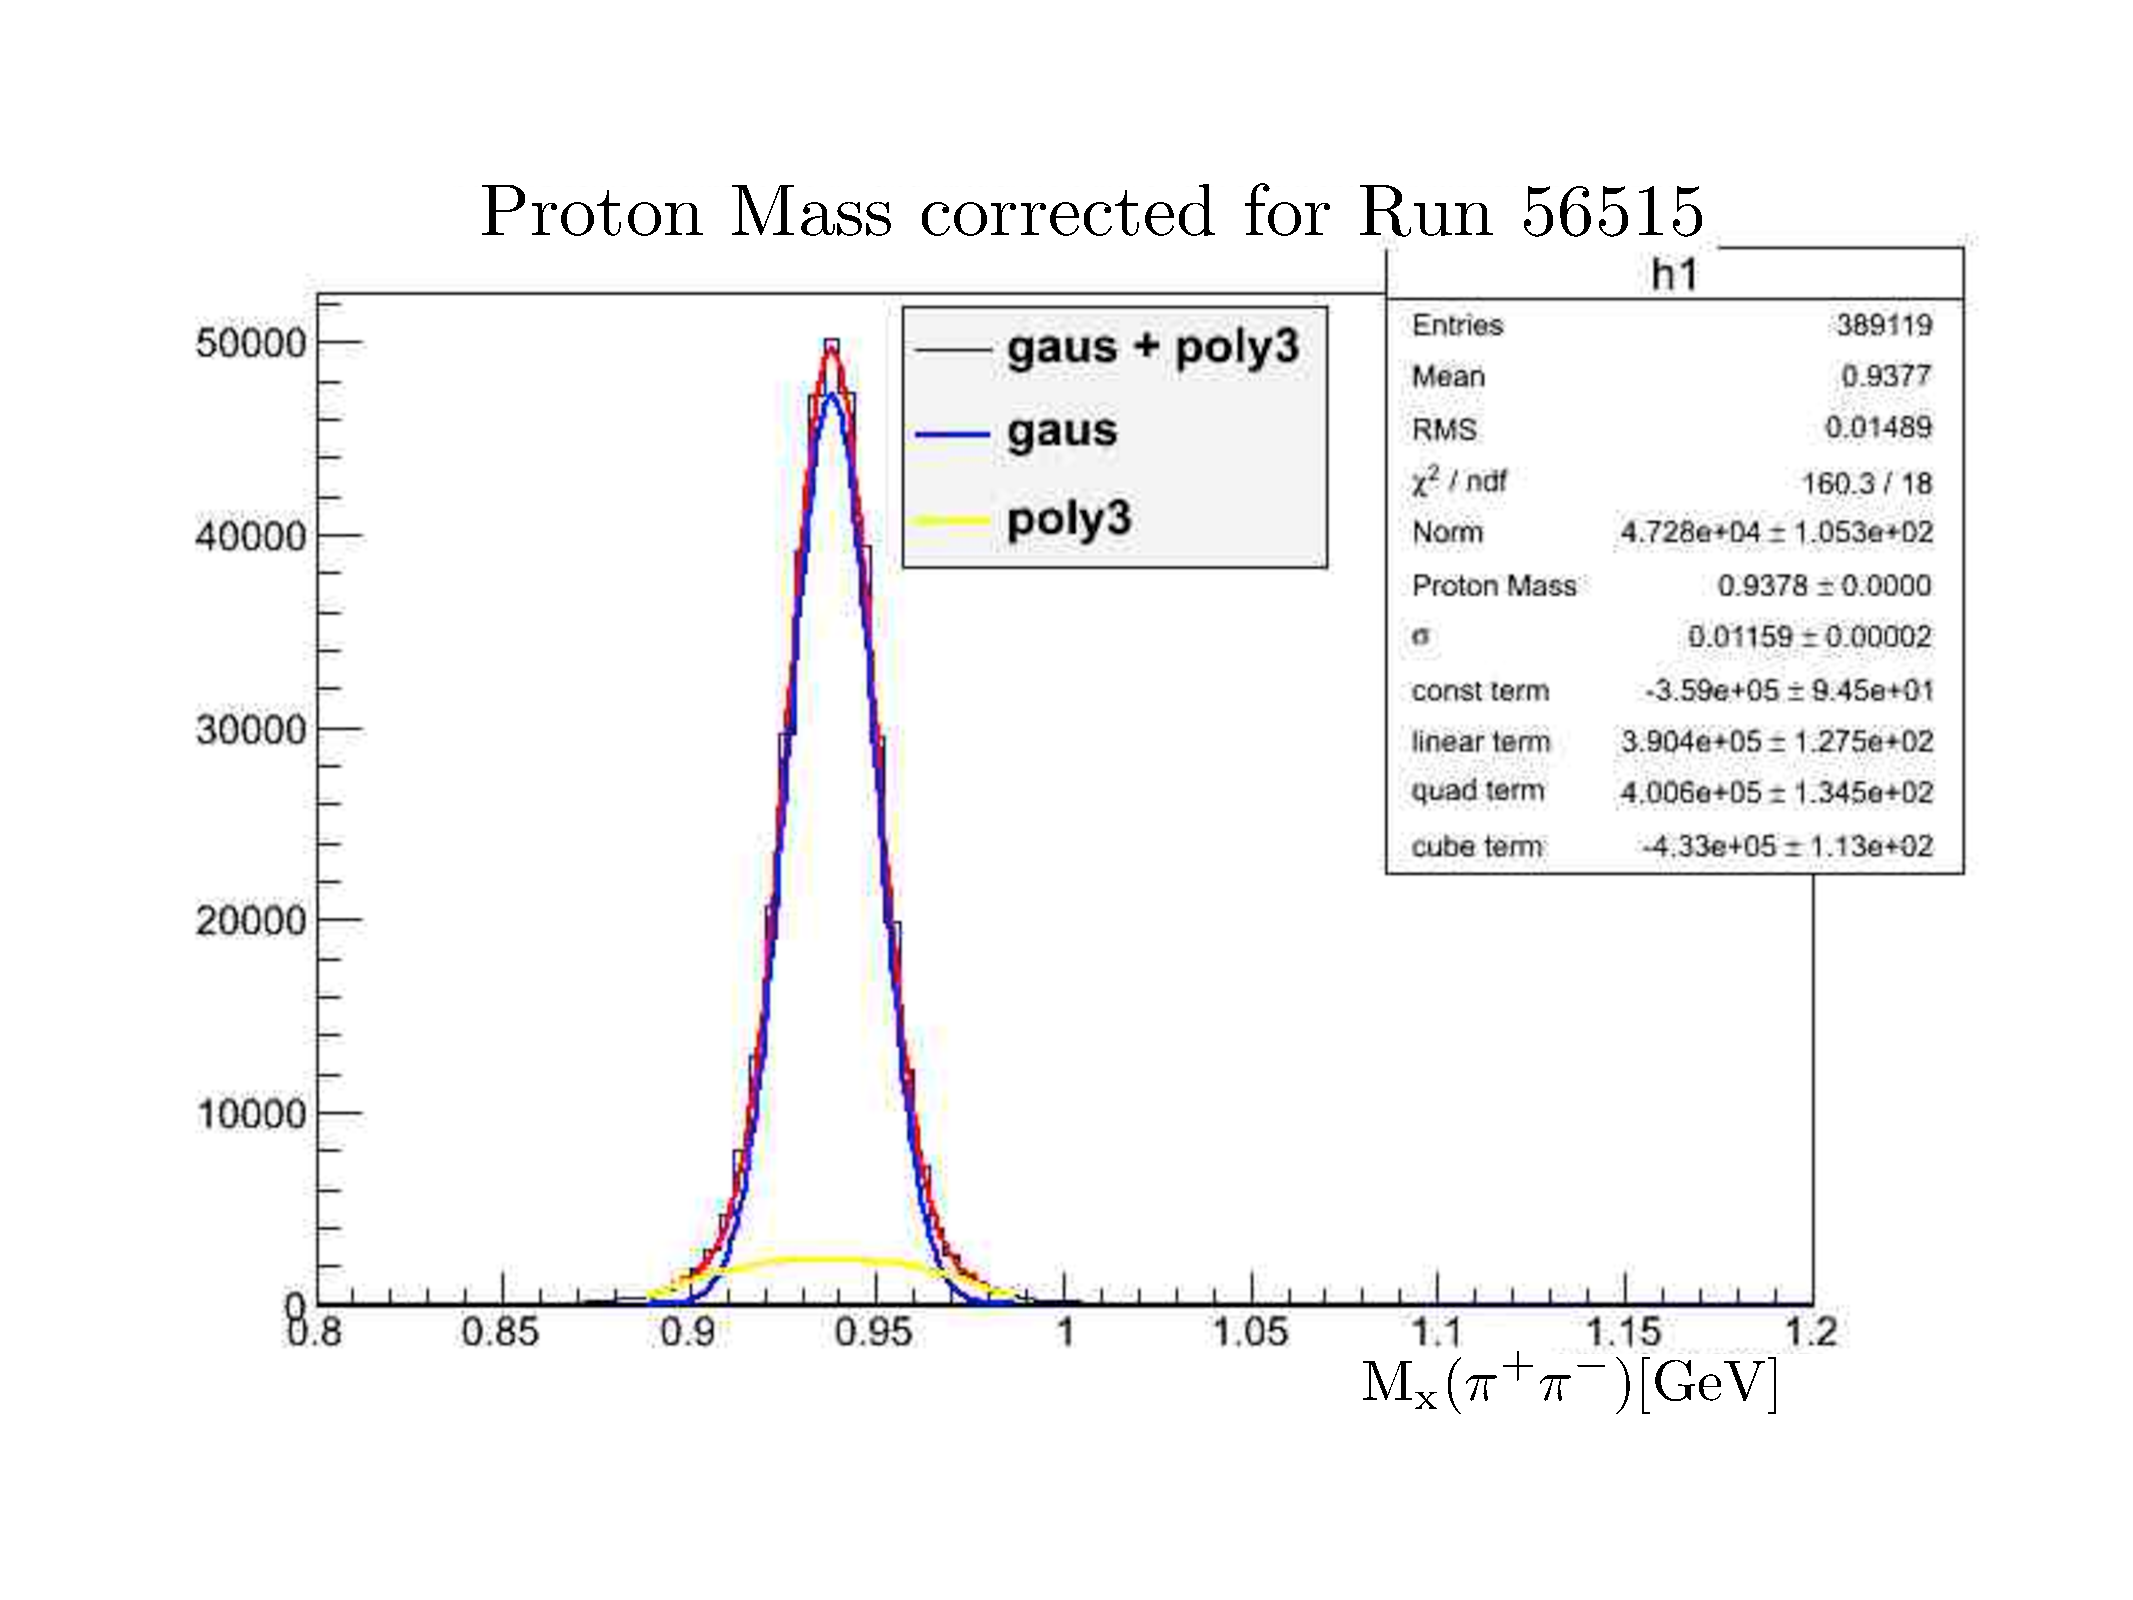
\includegraphics[width=\figwidth,height=0.7\hfigheight]{\figures/analysis/beam_correction/FixedmisssingmassII.pdf}
    \caption[Plot of proton mass for runs 56515 after beam correction was applied]{\label{fig:proton.fix} Plot of proton mass for runs 56515 after beam correction was applied.  \abbr{PDG} mass for the proton is 0.938272 GeV/c.}
    \end{center}\end{figure}
    
    \begin{figure}[h!]\begin{center}
    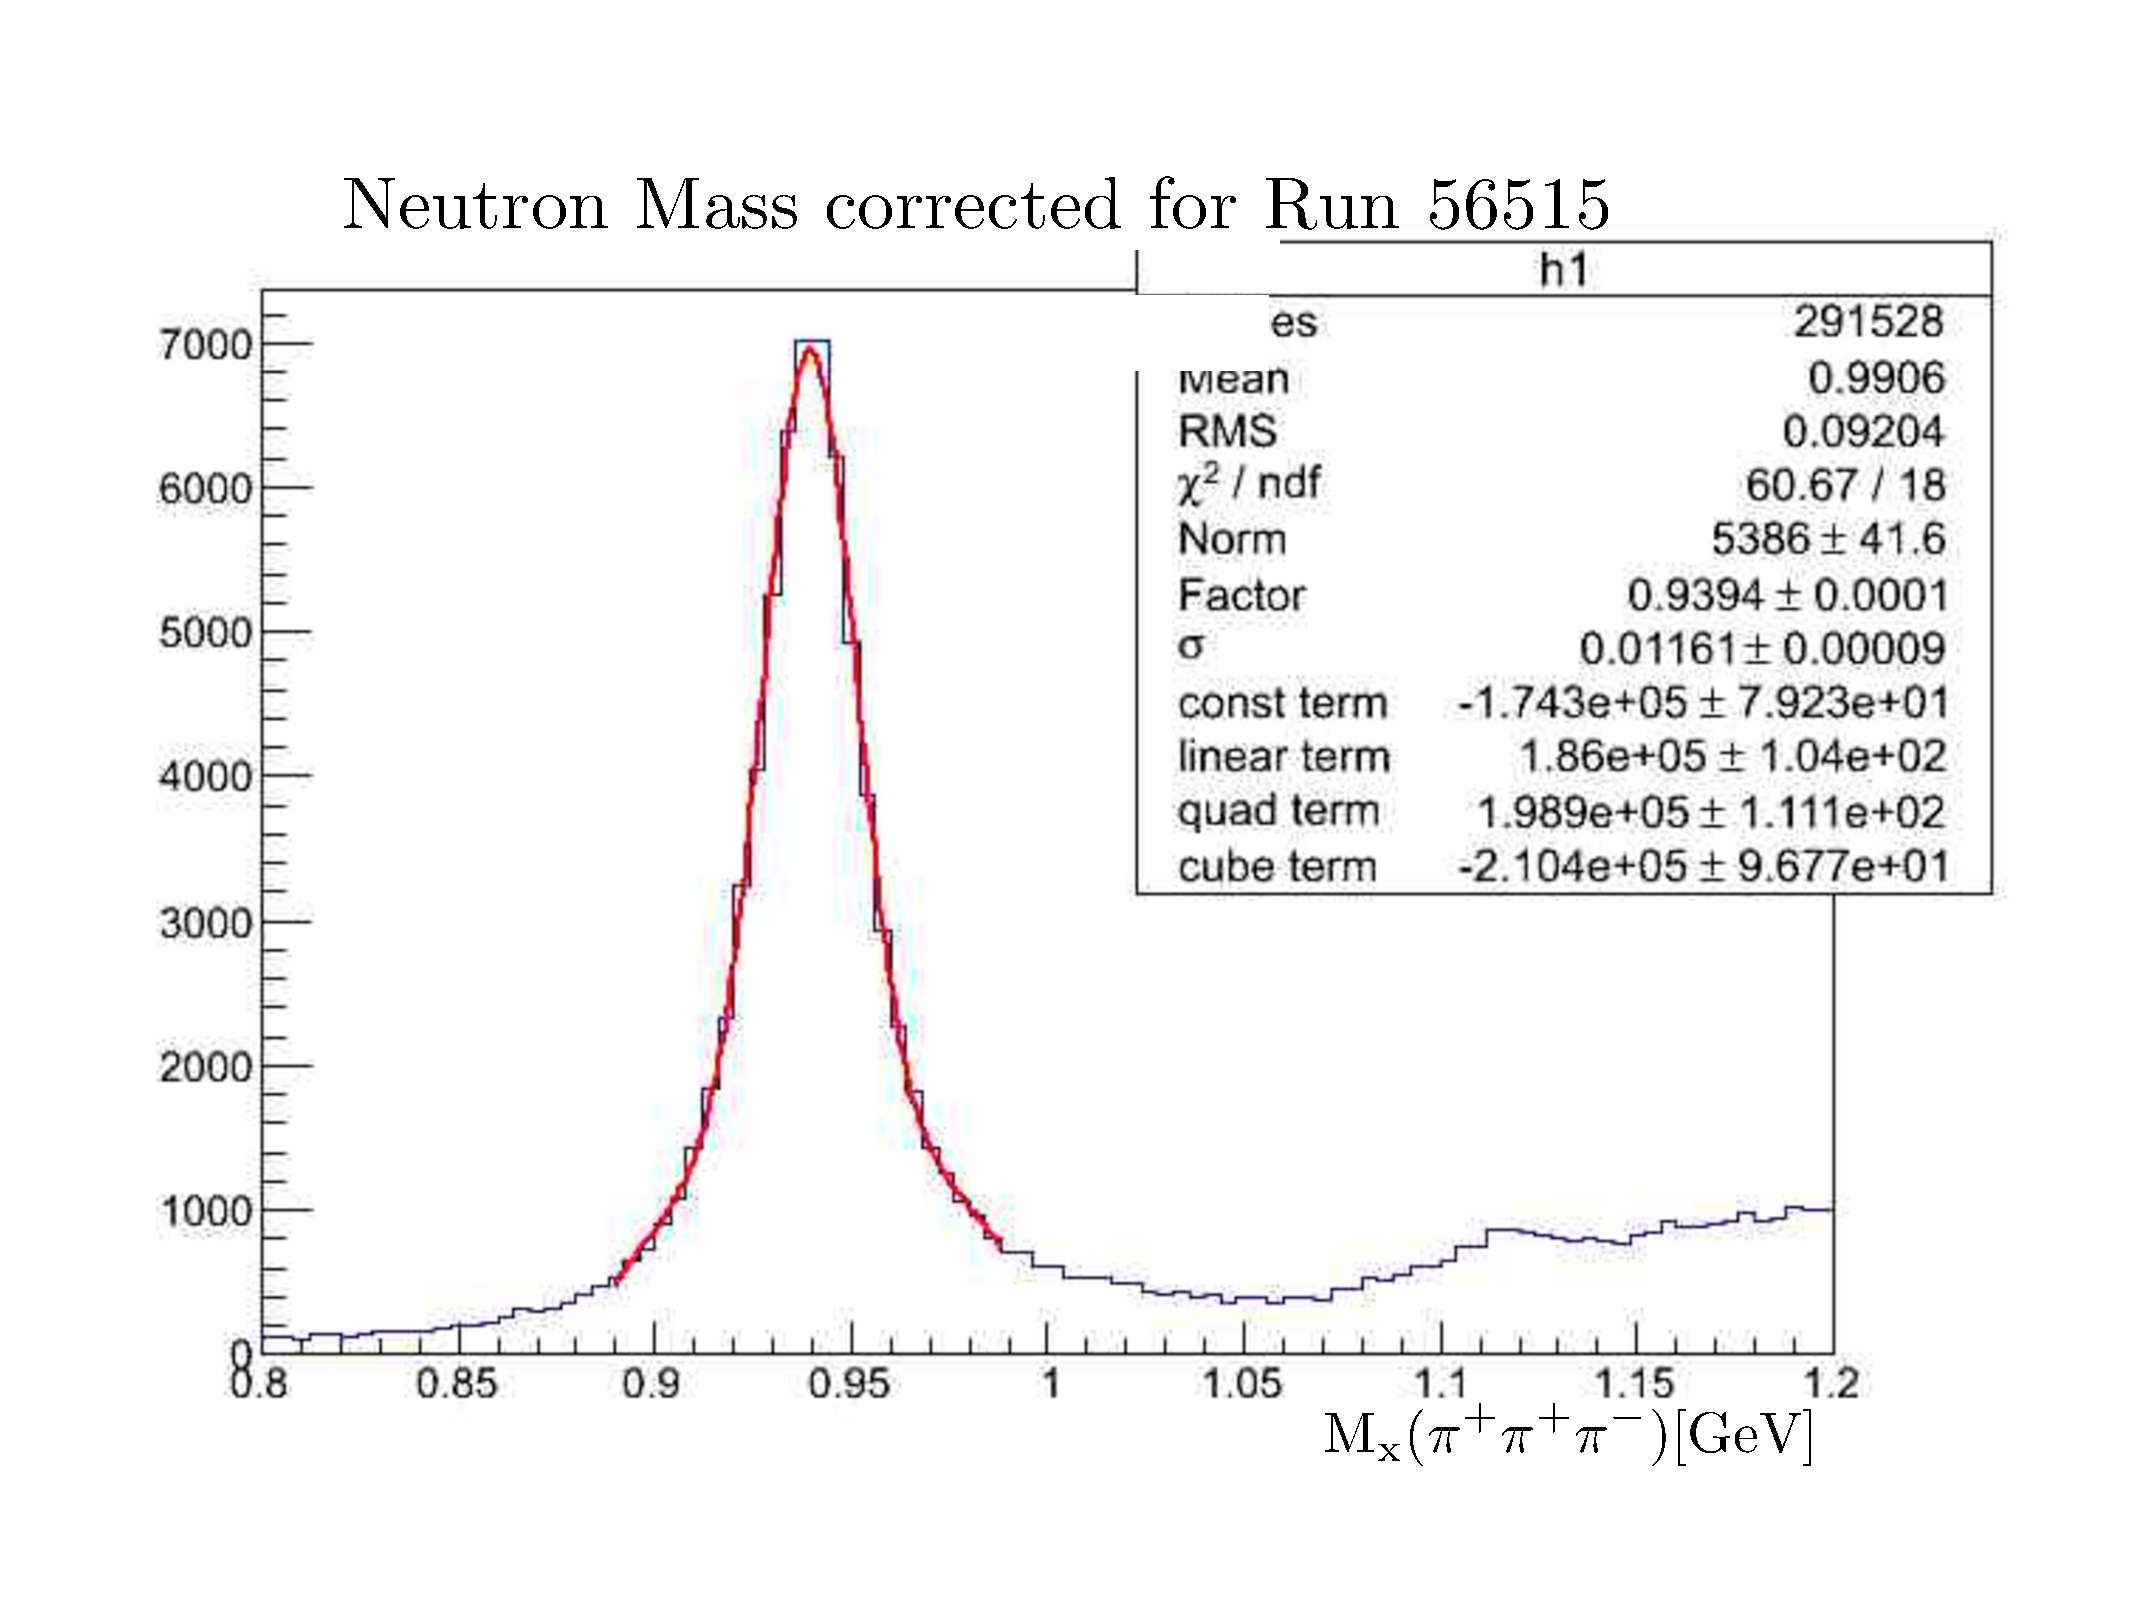
\includegraphics[width=\figwidth,height=0.7\hfigheight]{\figures/analysis/beam_correction/FixedmisssingmassneutronII.pdf}
    \caption[Plot of neutron mass for runs 56515 after beam correction was applied]{\label{fig:neutron.fix} Plot of neutron mass for runs 56515 after beam correction was applied.  \abbr{PDG} mass for the neutron is 0.939565 GeV/c.}
    \end{center}\end{figure}
    
    \begin{figure}[h!]\begin{center}
    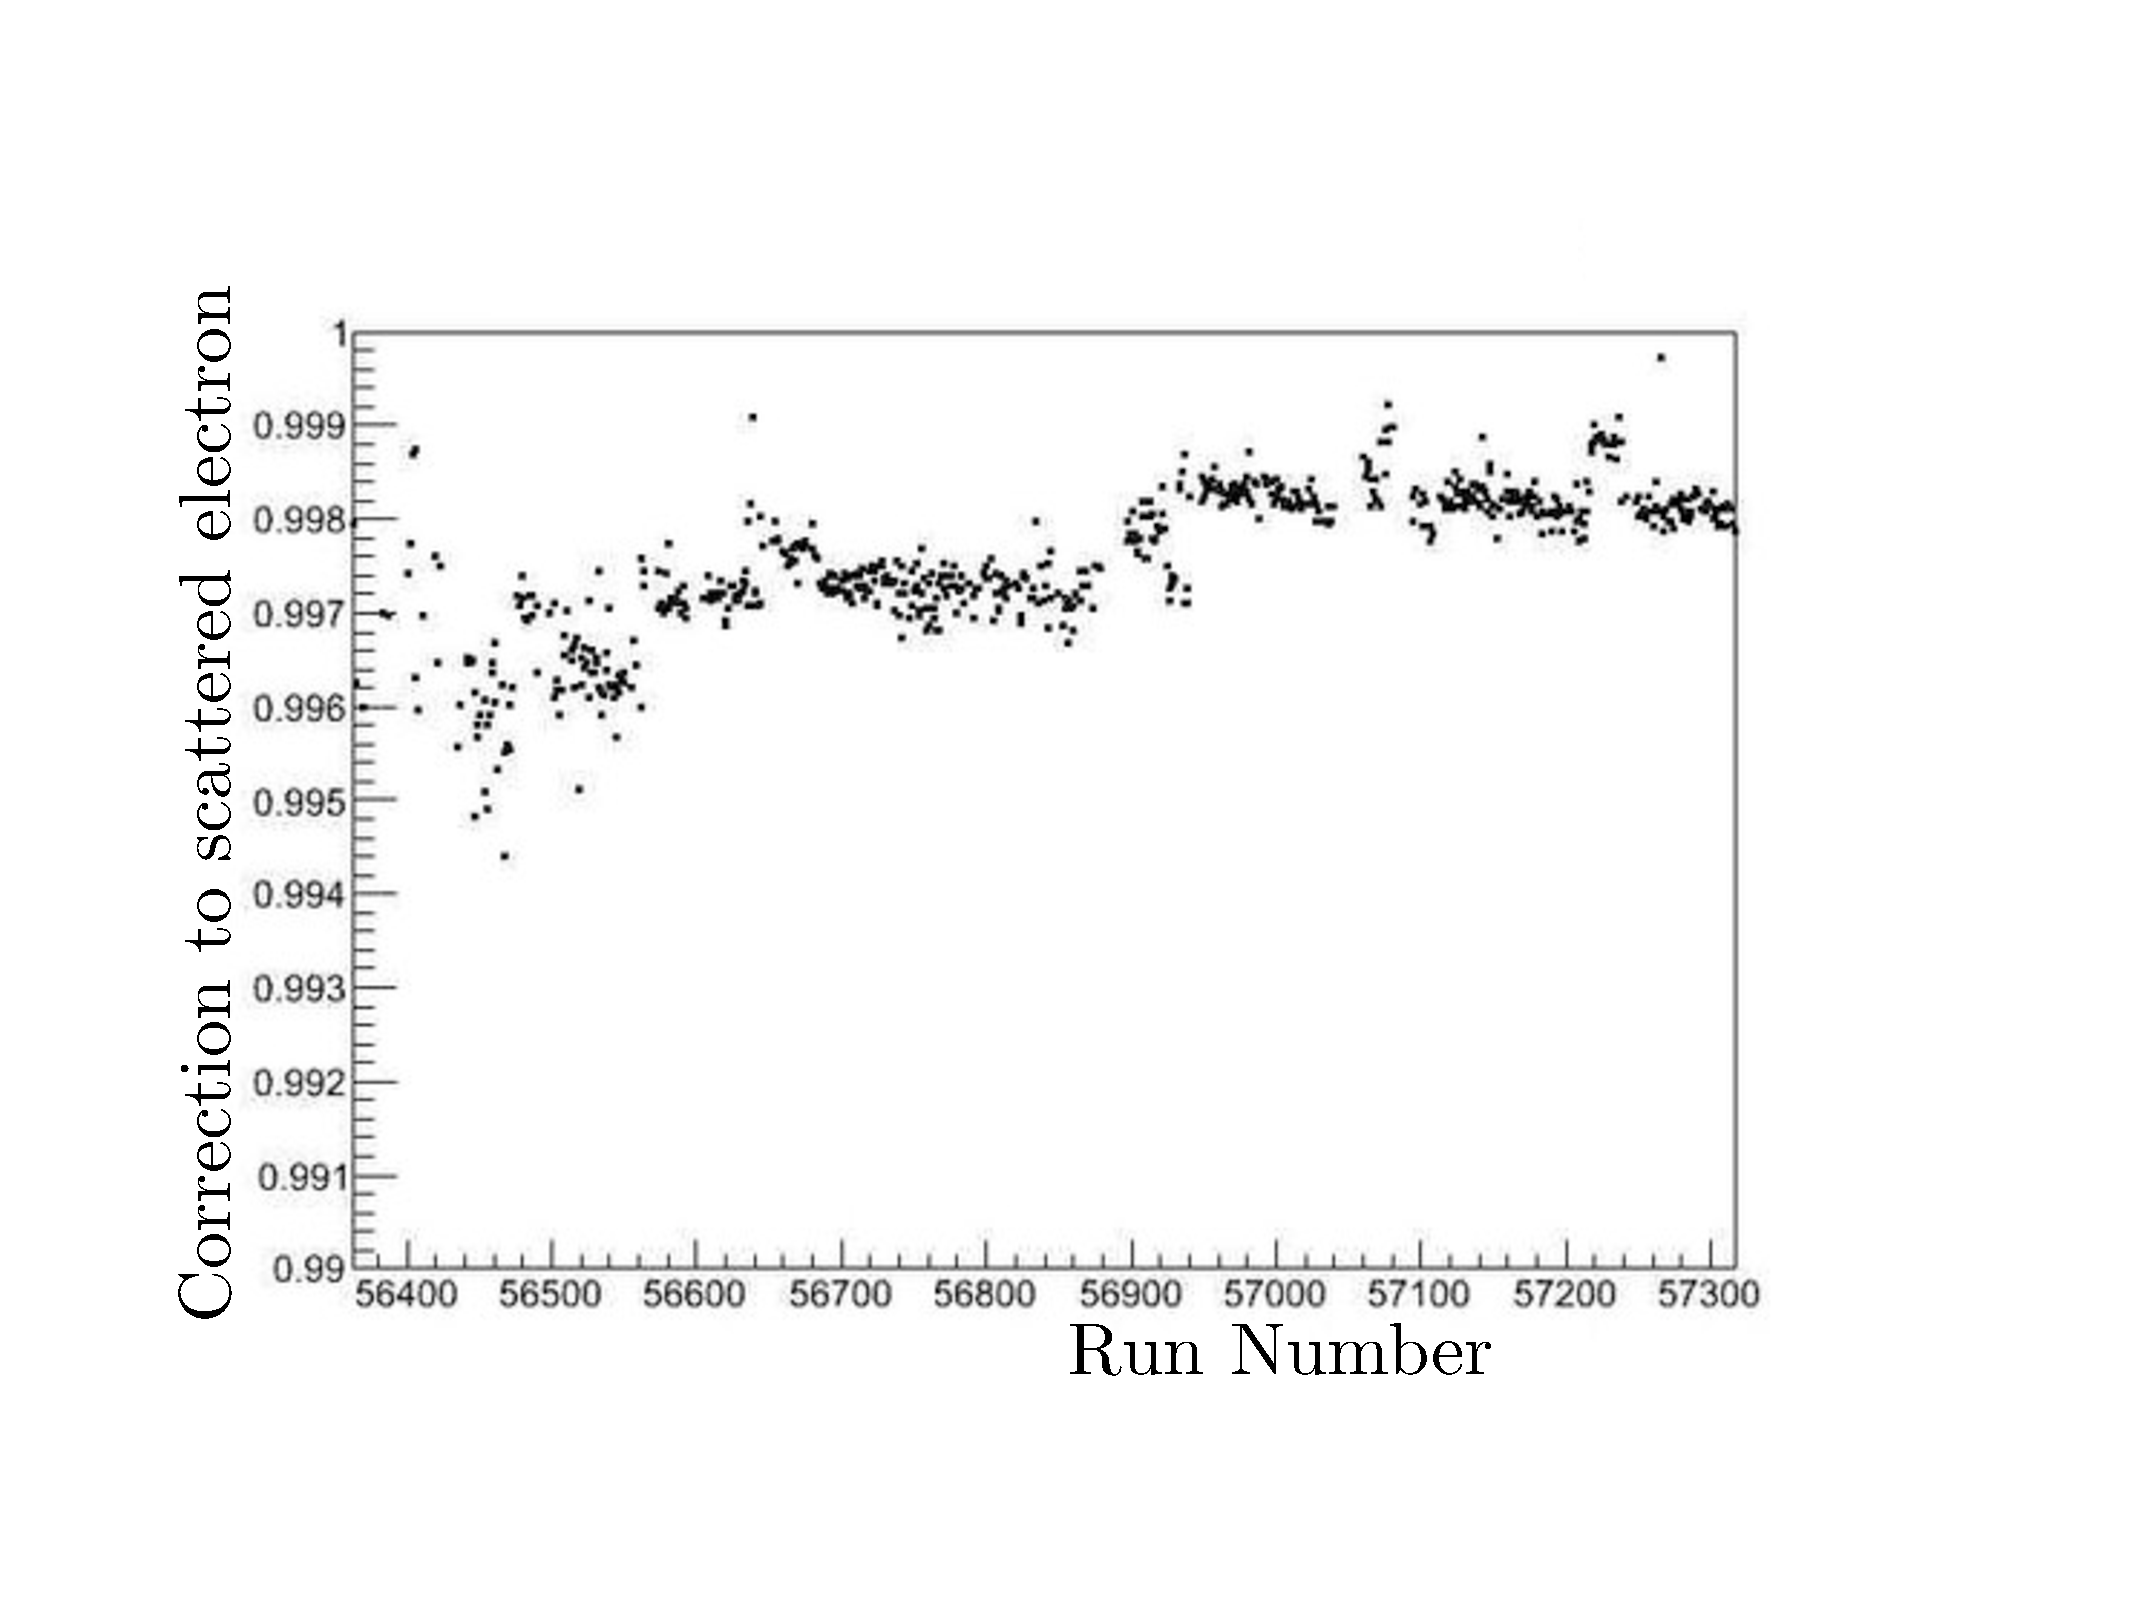
\includegraphics[width=\figwidth,height=0.7\hfigheight]{\figures/analysis/beam_correction/beam_cor.pdf}
    \caption[Plot of the correction factor $x$ as a function of run number]{\label{fig:beamcor.run} Plot of the correction factor $x$ as a function of run number.}
    \end{center}\end{figure}
    
    \begin{figure}[h!]\begin{center}
    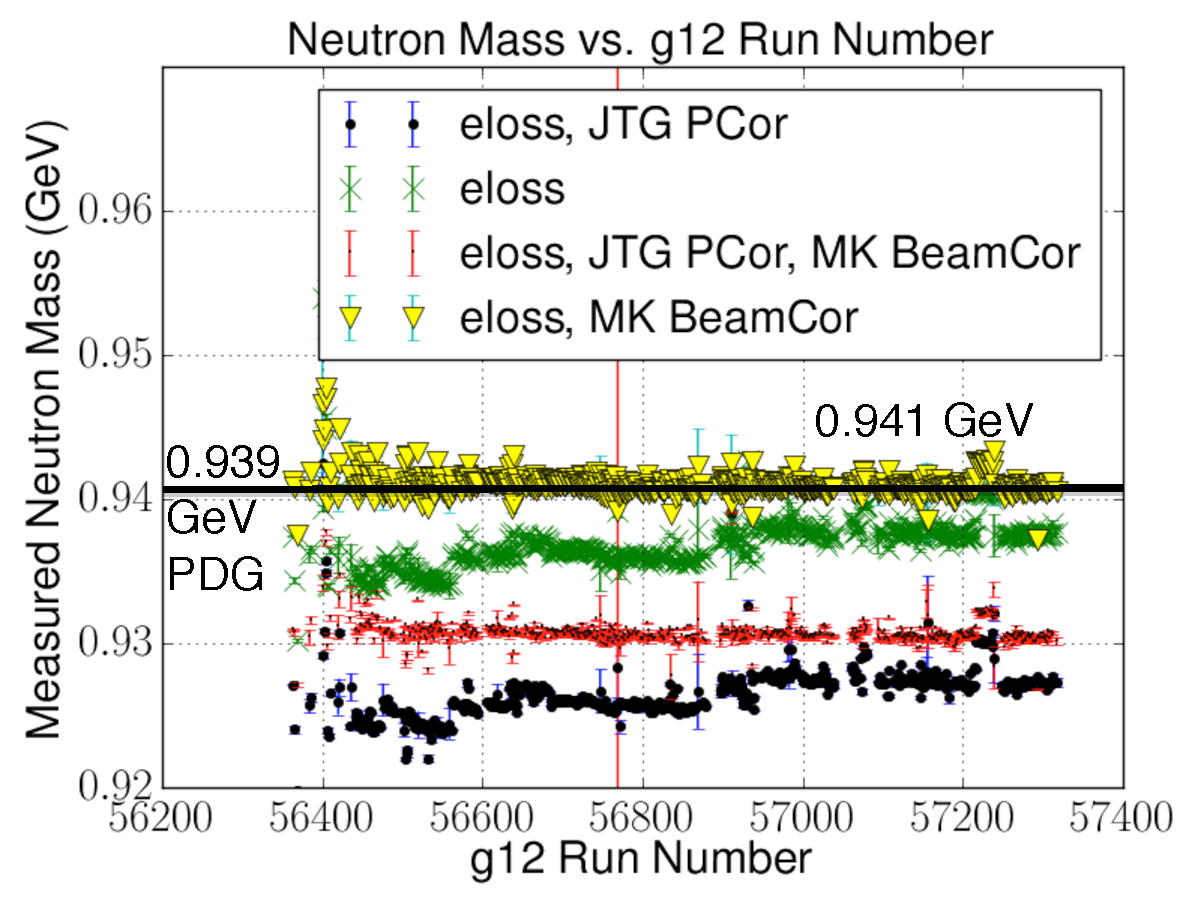
\includegraphics[width=\figwidth,height=0.7\hfigheight]{\figures/analysis/beam_correction/C3pi_allcorr_neutron_rxr.pdf}
    \caption[Plot of missing neutron mass vs. run number using various corrections]{\label{fig:neutron.fixall} Plot of missing neutron mass vs. run number using various corrections. The yellow triangles show a missing neutron mass with only ``energy-loss'' and beam correction applied (MK BeamCor) which was the only corrections needed to correct the \g12 data stream.}
    \end{center}\end{figure}
    
    %
    % Arne Freyberger
    
    \FloatBarrier
